\documentclass[a4paper]{book}
\usepackage{a4wide}
\usepackage{makeidx}
\usepackage{graphicx}
\usepackage{multicol}
\usepackage{float}
\usepackage{listings}
\usepackage{color}
\usepackage{textcomp}
\usepackage{alltt}
\usepackage[utf8]{inputenc}
\usepackage{doxygen}
\lstset{language=C++,inputencoding=utf8,basicstyle=\footnotesize,breaklines=true,breakatwhitespace=true,tabsize=8,numbers=left }
\makeindex
\setcounter{tocdepth}{3}
\renewcommand{\footrulewidth}{0.4pt}
\begin{document}
\begin{titlepage}
\vspace*{7cm}
\begin{center}
{\Large LABVIEW2LCIO \\[1ex]\large 1.0.0 }\\
\vspace*{1cm}
{\large Generated by Doxygen 1.6.1}\\
\vspace*{0.5cm}
<<<<<<< HEAD
{\small Thu Dec 14 00:30:26 2017}\\
=======
{\small Fri Dec 1 18:24:01 2017}\\
>>>>>>> 61ee8a49f17bf490f5d24a65bcc074f82aefb511
\end{center}
\end{titlepage}
\clearemptydoublepage
\pagenumbering{roman}
\tableofcontents
\clearemptydoublepage
\pagenumbering{arabic}
\chapter{Todo List}
\label{todo}
\label{todo__todo000001}
 
\begin{DoxyDescription}
\item[Global \doxyref{marlin::RootWriteEngine::getEngineName}{p.}{classmarlin_1_1RootWriteEngine_a31e38120fe60efcb15666fd569ba5862}()=0 ]fixme: should be const, but must be declared const in implementations too. Need to fix all existing engines?!? 
\end{DoxyDescription}
\chapter{Directory Hierarchy}
\section{Directories}
This directory hierarchy is sorted roughly, but not completely, alphabetically:\begin{DoxyCompactList}
\item \contentsline{section}{calice\_\-calib}{\pageref{dir_5116c8f7e4b5645f509e1533a2a6cce8}}{}
\begin{DoxyCompactList}
\item \contentsline{section}{fitmip}{\pageref{dir_8b66d6ab1bfe1b4e4607d2386115a489}}{}
\begin{DoxyCompactList}
\item \contentsline{section}{include}{\pageref{dir_a6f1c71feca9fe1ce77867768a90757d}}{}
\item \contentsline{section}{src}{\pageref{dir_d44fa2f799089ff9624f0a48581df711}}{}
\end{DoxyCompactList}
\end{DoxyCompactList}
\end{DoxyCompactList}

\chapter{Namespace Index}
\section{Namespace List}
Here is a list of all documented namespaces with brief descriptions:\begin{DoxyCompactList}
\item\contentsline{section}{{\bf CALICE} (Processor to read SLCIO EUDAQ files and sort them according to the BXID (now they are sorted in readout cycles) (either a separation between ECAL and AHCAL collections is done by EUDAQ) )}{\pageref{namespaceCALICE}}{}
\end{DoxyCompactList}

\chapter{Data Structure Index}
\section{Class List}
Here are the classes, structs, unions and interfaces with brief descriptions:\begin{DoxyCompactList}
\item\contentsline{section}{{\bf CALICE::multiCalibrator} (Processor to add PAR\_\-MULTI to the event and calibrate the threshold )}{\pageref{classCALICE_1_1multiCalibrator}}{}
\item\contentsline{section}{{\bf TConvolution} (ROOT class which generates the convolution of two functions )}{\pageref{classTConvolution}}{}
\end{DoxyCompactList}

\chapter{Directory Documentation}
\section{/afs/desy.de/user/t/torimart/work/CosmiTestLCIO/labview\_\-converter/raw2lcio/include/ Directory Reference}
\label{dir_55fca3d99a726b7ca1a5be083ce2821c}\index{/afs/desy.de/user/t/torimart/work/CosmiTestLCIO/labview\_\-converter/raw2lcio/include/ Directory Reference@{/afs/desy.de/user/t/torimart/work/CosmiTestLCIO/labview\_\-converter/raw2lcio/include/ Directory Reference}}
\subsection*{Files}
\begin{DoxyCompactItemize}
\item 
file {\bfseries BIFBlock.hh}
\item 
file {\bfseries EUDAQBlock.hh}
\item 
file {\bfseries EUDAQBlock2016.hh}
\item 
file {\bfseries EUDAQEventBuilder.hh}
\item 
file {\bfseries EUDAQEventBuilder2016.hh}
\item 
file {\bfseries EUDAQEventBuilder2016\_\-woBIF.hh}
\item 
file {\bfseries EUDAQTempSensorBlock.hh}
\item 
file {\bfseries EventChecker.hh}
\item 
file {\bfseries HBUtemperatureBlock.hh}
\item 
file {\bfseries hodoscopeBlock.hh}
\item 
file {\bfseries LabviewBlock.hh}
\item 
file {\bfseries LabviewBlock2.hh}
\item 
file {\bfseries LabviewConverter.hh}
\item 
file {\bfseries LabviewConverter2.hh}
\item 
file {\bfseries LConverter.hh}
\item 
file {\bfseries RootTreeGenerator.hh}
\item 
file {\bfseries RootTreeGenerator2.hh}
\item 
file {\bfseries RootTreeGenerator3.hh}
\item 
file {\bfseries RootTreeGeneratorEUDAQ2016.hh}
\item 
file {\bfseries RootWriteEngine.hh}
\item 
file {\bfseries TempRootTreeGenerator.hh}
\item 
file {\bfseries TempSensorBlock.hh}
\item 
file {\bfseries TempSensorBlock2.hh}
\item 
file {\bfseries TempSensorBlockOld.hh}
\end{DoxyCompactItemize}

\section{/afs/desy.de/user/t/torimart/work/CosmiTestLCIO/labview\_\-converter/ Directory Reference}
\label{dir_c5b743f48f9eb5a75f6b18e12f728180}\index{/afs/desy.de/user/t/torimart/work/CosmiTestLCIO/labview\_\-converter/ Directory Reference@{/afs/desy.de/user/t/torimart/work/CosmiTestLCIO/labview\_\-converter/ Directory Reference}}
\subsection*{Directories}
\begin{DoxyCompactItemize}
\item 
directory {\bf raw2lcio}
\end{DoxyCompactItemize}

\section{/afs/desy.de/user/t/torimart/work/CosmiTestLCIO/labview\_\-converter/raw2lcio/ Directory Reference}
\label{dir_3900b01e79db89eeef685b93f5dff5d9}\index{/afs/desy.de/user/t/torimart/work/CosmiTestLCIO/labview\_\-converter/raw2lcio/ Directory Reference@{/afs/desy.de/user/t/torimart/work/CosmiTestLCIO/labview\_\-converter/raw2lcio/ Directory Reference}}
\subsection*{Directories}
\begin{DoxyCompactItemize}
\item 
directory {\bf include}
\item 
directory {\bf src}
\end{DoxyCompactItemize}

\section{/afs/desy.de/user/t/torimart/work/CosmiTestLCIO/labview\_\-converter/raw2lcio/src/ Directory Reference}
\label{dir_f5886fba70a35cb1e14992eb08dc189c}\index{/afs/desy.de/user/t/torimart/work/CosmiTestLCIO/labview\_\-converter/raw2lcio/src/ Directory Reference@{/afs/desy.de/user/t/torimart/work/CosmiTestLCIO/labview\_\-converter/raw2lcio/src/ Directory Reference}}
\subsection*{Files}
\begin{DoxyCompactItemize}
\item 
file {\bfseries EUDAQEventBuilder.cc}
\item 
file {\bfseries EUDAQEventBuilder2016.cc}
\item 
file {\bfseries EUDAQEventBuilder2016\_\-woBIF.cc}
\item 
file {\bfseries EventChecker.cc}
\item 
file {\bfseries LabviewConverter.cc}
\item 
file {\bfseries LabviewConverter2.cc}
\item 
file {\bfseries RootTreeGenerator.cc}
\item 
file {\bfseries RootTreeGenerator2.cc}
\item 
file {\bfseries RootTreeGenerator3.cc}
\item 
file {\bfseries RootTreeGeneratorEUDAQ2016.cc}
\item 
file {\bfseries TempRootTreeGenerator.cc}
\end{DoxyCompactItemize}

\chapter{Namespace Documentation}
\section{CALICE Namespace Reference}
\label{namespaceCALICE}\index{CALICE@{CALICE}}


Processor to read SLCIO EUDAQ files and sort them according to the BXID Then do the AHCAL-\/BIF Offset calibration by counting the number of correlated events (either a separation between ECAL and AHCAL collections is done by EUDAQ).  
\subsection*{Data Structures}
\begin{DoxyCompactItemize}
\item 
class {\bf Ahc2GainCalibrator}
\item 
class {\bf Ahc2OffsetCalibrator}
\begin{DoxyCompactList}\small\item\em Processor to read SLCIO EUDAQ files and sort them according to the BXID Then do the AHCAL-\/BIF Offset calibration by counting the number of correlated events (either a separation between ECAL and AHCAL collections is done by EUDAQ). \item\end{DoxyCompactList}\item 
class {\bf Ahc2PedestalCalibrator}
\item 
class {\bf AngleTrackFinder}
\begin{DoxyCompactList}\small\item\em Processor to extract MIP calibrations from muon beam runs. \item\end{DoxyCompactList}\item 
class {\bf MipTrackFinder}
\begin{DoxyCompactList}\small\item\em Processor to extract MIP calibrations from muon beam runs. \item\end{DoxyCompactList}\item 
class {\bf SingleCellAnalysis}
\begin{DoxyCompactList}\small\item\em Processor for analysing cellwise properties like mean signal, RMS, hit frequency, . \item\end{DoxyCompactList}\end{DoxyCompactItemize}
\subsection*{Functions}
\begin{DoxyCompactItemize}
\item 
double {\bfseries MultiGaus} (double $\ast$x, double $\ast$par)\label{namespaceCALICE_ab027e03d90dee39729ce0c0ff8524bfb}

\end{DoxyCompactItemize}
\subsection*{Variables}
\begin{DoxyCompactItemize}
\item 
{\bf Ahc2GainCalibrator} {\bfseries aAhc2GainCalibrator}\label{namespaceCALICE_aff0f779ea231c17c5f3447d5f1c85c5a}

\item 
{\bf Ahc2OffsetCalibrator} {\bfseries aAhc2OffsetCalibrator}\label{namespaceCALICE_a0dfd57d58d988a974ce3c87364e65fc1}

\item 
{\bf Ahc2PedestalCalibrator} {\bfseries aAhc2PedestalCalibrator}\label{namespaceCALICE_abe03f653dfffe06ae6550343edbbb184}

\item 
{\bf AngleTrackFinder} {\bfseries AngleTrackFinder}\label{namespaceCALICE_a3a6925ca17e1f05cc97e625f7edd5ed5}

\item 
{\bf MipTrackFinder} {\bfseries aMipTrackFinder}\label{namespaceCALICE_a63db13b96d3be485b4c57ba60db44bdd}

\item 
{\bf SingleCellAnalysis} {\bfseries aSingleCellAnalysis}\label{namespaceCALICE_a0c491b351d33b91639df2101f7725139}

\end{DoxyCompactItemize}


\subsection{Detailed Description}
Processor to read SLCIO EUDAQ files and sort them according to the BXID Then do the AHCAL-\/BIF Offset calibration by counting the number of correlated events (either a separation between ECAL and AHCAL collections is done by EUDAQ). \begin{DoxyAuthor}{Author}
E. Brianne, DESY Hamburg 
\end{DoxyAuthor}
\begin{DoxyDate}{Date}
May 2016 Created for 2016 testbeams EUDAQ data format and AHCAL-\/BIF Offset calibration. 
\end{DoxyDate}

\chapter{Data Structure Documentation}
\section{CALICE::BIFBlock Class Reference}
\label{classCALICE_1_1BIFBlock}\index{CALICE::BIFBlock@{CALICE::BIFBlock}}


Class for the SLCIO EUDAQ BIF Data as acquired by the EUDAQ system.  


{\ttfamily \#include $<$BIFBlock.hh$>$}\subsection*{Public Member Functions}
\begin{DoxyCompactItemize}
\item 
{\bf BIFBlock} ()\label{classCALICE_1_1BIFBlock_a07e68d7015e5012ce8d2c6fcff0cb1ba}

\begin{DoxyCompactList}\small\item\em Constructor. \item\end{DoxyCompactList}\item 
{\bf BIFBlock} (int TriggerSource, int BXID\_\-BIF, float Time\_\-BIF)\label{classCALICE_1_1BIFBlock_ac7d82de3658f1c613a08072450a85fb0}

\begin{DoxyCompactList}\small\item\em Convenient constructor. \item\end{DoxyCompactList}\item 
virtual {\bf $\sim$BIFBlock} ()\label{classCALICE_1_1BIFBlock_a66d7f8a31626549b3c7b1b117cf70ae1}

\begin{DoxyCompactList}\small\item\em Destructor. \item\end{DoxyCompactList}\item 
void {\bf print} (std::ostream \&os, int)\label{classCALICE_1_1BIFBlock_a95fa0c06efa6a87da8cf1e8380072cde}

\begin{DoxyCompactList}\small\item\em Convenient print method. \item\end{DoxyCompactList}\item 
void {\bf setTriggerSource} (int TriggerSource)\label{classCALICE_1_1BIFBlock_a011c8771a288f584e02335821ecd2aa9}

\begin{DoxyCompactList}\small\item\em Set Trigger type. \item\end{DoxyCompactList}\item 
void {\bf setBXID} (int BXID\_\-BIF)\label{classCALICE_1_1BIFBlock_a089b2f4c9b362e0f95e8942f559bdfcd}

\begin{DoxyCompactList}\small\item\em Set BXID of the BIF Trigger. \item\end{DoxyCompactList}\item 
void {\bf setTime} (float Time\_\-BIF)\label{classCALICE_1_1BIFBlock_aa7286d6fe67c4c941537a0f156812247}

\begin{DoxyCompactList}\small\item\em Set Time of the BIF Trigger. \item\end{DoxyCompactList}\item 
const int {\bf getTriggerSource} () const \label{classCALICE_1_1BIFBlock_a27cde06f0406d3908efc8ec0b047332e}

\begin{DoxyCompactList}\small\item\em Get Trigger type. \item\end{DoxyCompactList}\item 
const int {\bf getBXID} () const \label{classCALICE_1_1BIFBlock_a7104742c4a7d0a3a17b0e195371ccf4c}

\begin{DoxyCompactList}\small\item\em Get BXID of the BIF Trigger. \item\end{DoxyCompactList}\item 
const float {\bf getTime} () const \label{classCALICE_1_1BIFBlock_a78df0b79c7631dd015db810eb5e653cd}

\begin{DoxyCompactList}\small\item\em Get Time of the BIF Trigger. \item\end{DoxyCompactList}\item 
const std::string {\bf getTypeName} () const \label{classCALICE_1_1BIFBlock_afedd9050ce2f4ae465c0c5c69ace43e9}

\begin{DoxyCompactList}\small\item\em Return the type of the class. \item\end{DoxyCompactList}\item 
const std::string {\bf getDataDescription} () const \label{classCALICE_1_1BIFBlock_a103f8aa8e9bc3073acfd2adb865342f0}

\begin{DoxyCompactList}\small\item\em Return a brief description of the data members. \item\end{DoxyCompactList}\end{DoxyCompactItemize}


\subsection{Detailed Description}
Class for the SLCIO EUDAQ BIF Data as acquired by the EUDAQ system. \begin{DoxyAuthor}{Author}
E.Brianne @ DESY Hamburg 
\end{DoxyAuthor}
\begin{DoxyDate}{Date}
May 2016 Created for 2016 testbeams EUDAQ data format. 
\end{DoxyDate}


Definition at line 37 of file BIFBlock.hh.

The documentation for this class was generated from the following file:\begin{DoxyCompactItemize}
\item 
BIFBlock.hh\end{DoxyCompactItemize}

\section{CALICE::EUDAQBlock Class Reference}
\label{classCALICE_1_1EUDAQBlock}\index{CALICE::EUDAQBlock@{CALICE::EUDAQBlock}}


Class for the SLCIO EUDAQ Data as acquired by the EUDAQ system.  


{\ttfamily \#include $<$EUDAQBlock.hh$>$}\subsection*{Public Member Functions}
\begin{DoxyCompactItemize}
\item 
{\bf EUDAQBlock} (int CycleNr, int BunchXID, int ChipID, int EvtNr, int Channel, int TDC, int ADC, int HitBit, int GainBit)\label{classCALICE_1_1EUDAQBlock_a2576c4ead40588d8ea075d9629926ce3}

\begin{DoxyCompactList}\small\item\em Convenient c'tor. \item\end{DoxyCompactList}\item 
{\bf EUDAQBlock} (LCObject $\ast$obj)\label{classCALICE_1_1EUDAQBlock_adf2c1a0b660a881f637ae260033b2068}

\begin{DoxyCompactList}\small\item\em 'Copy constructor' needed to interpret LCCollection read from file/database. \item\end{DoxyCompactList}\item 
virtual {\bf $\sim$EUDAQBlock} ()\label{classCALICE_1_1EUDAQBlock_ac009640c79883d5b236ffa1f01a4da08}

\begin{DoxyCompactList}\small\item\em Important for memory handling. \item\end{DoxyCompactList}\item 
int {\bf GetCycleNr} () const \label{classCALICE_1_1EUDAQBlock_a7267f8e75e5ee64c2b558a1cb58b5370}

\begin{DoxyCompactList}\small\item\em get the CycleNr. \item\end{DoxyCompactList}\item 
int {\bf GetBunchXID} () const \label{classCALICE_1_1EUDAQBlock_a9e868629e66c71f4a5086ee4515d75a6}

\begin{DoxyCompactList}\small\item\em get the BunchXID. \item\end{DoxyCompactList}\item 
int {\bf GetChipID} () const \label{classCALICE_1_1EUDAQBlock_a29e7cb6cea36a5726c185af80f602a04}

\begin{DoxyCompactList}\small\item\em get the ChipID. \item\end{DoxyCompactList}\item 
int {\bf GetEvtNr} () const \label{classCALICE_1_1EUDAQBlock_a274bfd6d90f473f1875fd2045268e27f}

\begin{DoxyCompactList}\small\item\em get the EvtNr. \item\end{DoxyCompactList}\item 
int {\bf GetChannel} () const \label{classCALICE_1_1EUDAQBlock_a5665cd40d1deb96c634a7e131be981a8}

\begin{DoxyCompactList}\small\item\em get the Channel. \item\end{DoxyCompactList}\item 
int {\bf GetTDC} () const \label{classCALICE_1_1EUDAQBlock_a66a6c244efdc2357b15350e778f98e56}

\begin{DoxyCompactList}\small\item\em get the TDC. \item\end{DoxyCompactList}\item 
int {\bf GetADC} () const \label{classCALICE_1_1EUDAQBlock_ac6ad7fd2adcc72ed2aa861eac4d89a0d}

\begin{DoxyCompactList}\small\item\em get the ADC. \item\end{DoxyCompactList}\item 
int {\bf GetHitBit} () const \label{classCALICE_1_1EUDAQBlock_a42be25f91cc050d64bba79ff4718b5c4}

\begin{DoxyCompactList}\small\item\em get the HitBit. \item\end{DoxyCompactList}\item 
int {\bf GetGainBit} () const \label{classCALICE_1_1EUDAQBlock_ac2573362003677a183343529bc63d74c}

\begin{DoxyCompactList}\small\item\em get the GainBit. \item\end{DoxyCompactList}\item 
void {\bf print} (std::ostream \&os, int)\label{classCALICE_1_1EUDAQBlock_a4f65b14367aa1123dd7a8a74e5d24ee1}

\begin{DoxyCompactList}\small\item\em Convenient print method. \item\end{DoxyCompactList}\item 
const std::string {\bf getTypeName} () const \label{classCALICE_1_1EUDAQBlock_aea8613f7fc6cbb4bcbc0294a020d3eca}

\begin{DoxyCompactList}\small\item\em Return the type of the class. \item\end{DoxyCompactList}\item 
const std::string {\bf getDataDescription} () const \label{classCALICE_1_1EUDAQBlock_a48d80a041501c9eaada74c500d78074c}

\begin{DoxyCompactList}\small\item\em Return a brief description of the data members. \item\end{DoxyCompactList}\end{DoxyCompactItemize}


\subsection{Detailed Description}
Class for the SLCIO EUDAQ Data as acquired by the EUDAQ system. \begin{DoxyAuthor}{Author}
A. Irles, based on the \doxyref{LabviewBlock2}{p.}{classCALICE_1_1LabviewBlock2} writen by S. Lu DESY Hamburg 
\end{DoxyAuthor}
\begin{DoxyDate}{Date}
May 20 2015 Created for 2015 testbeams EUDAQ data format. 
\end{DoxyDate}


Definition at line 23 of file EUDAQBlock.hh.

The documentation for this class was generated from the following file:\begin{DoxyCompactItemize}
\item 
EUDAQBlock.hh\end{DoxyCompactItemize}

\section{CALICE::EUDAQBlock2016 Class Reference}
\label{classCALICE_1_1EUDAQBlock2016}\index{CALICE::EUDAQBlock2016@{CALICE::EUDAQBlock2016}}


Class for the SLCIO EUDAQ Data as acquired by the EUDAQ system.  


{\ttfamily \#include $<$EUDAQBlock2016.hh$>$}\subsection*{Public Member Functions}
\begin{DoxyCompactItemize}
\item 
{\bf EUDAQBlock2016} (int CycleNr, int BunchXID, int EvtNr, int ChipID, int NChannels, int TDC\_\-0, int TDC\_\-1, int TDC\_\-2, int TDC\_\-3, int TDC\_\-4, int TDC\_\-5, int TDC\_\-6, int TDC\_\-7, int TDC\_\-8, int TDC\_\-9, int TDC\_\-10, int TDC\_\-11, int TDC\_\-12, int TDC\_\-13, int TDC\_\-14, int TDC\_\-15, int TDC\_\-16, int TDC\_\-17, int TDC\_\-18, int TDC\_\-19, int TDC\_\-20, int TDC\_\-21, int TDC\_\-22, int TDC\_\-23, int TDC\_\-24, int TDC\_\-25, int TDC\_\-26, int TDC\_\-27, int TDC\_\-28, int TDC\_\-29, int TDC\_\-30, int TDC\_\-31, int TDC\_\-32, int TDC\_\-33, int TDC\_\-34, int TDC\_\-35, int ADC\_\-0, int ADC\_\-1, int ADC\_\-2, int ADC\_\-3, int ADC\_\-4, int ADC\_\-5, int ADC\_\-6, int ADC\_\-7, int ADC\_\-8, int ADC\_\-9, int ADC\_\-10, int ADC\_\-11, int ADC\_\-12, int ADC\_\-13, int ADC\_\-14, int ADC\_\-15, int ADC\_\-16, int ADC\_\-17, int ADC\_\-18, int ADC\_\-19, int ADC\_\-20, int ADC\_\-21, int ADC\_\-22, int ADC\_\-23, int ADC\_\-24, int ADC\_\-25, int ADC\_\-26, int ADC\_\-27, int ADC\_\-28, int ADC\_\-29, int ADC\_\-30, int ADC\_\-31, int ADC\_\-32, int ADC\_\-33, int ADC\_\-34, int ADC\_\-35)\label{classCALICE_1_1EUDAQBlock2016_a695944edb5478e333e57bdf36b550cfe}

\begin{DoxyCompactList}\small\item\em Very ugly constructor because we use a Generic Object with many integers. \item\end{DoxyCompactList}\item 
{\bf EUDAQBlock2016} (LCObject $\ast$obj)\label{classCALICE_1_1EUDAQBlock2016_a69846d216e879d4d09388d712444ed6f}

\begin{DoxyCompactList}\small\item\em 'Copy constructor' needed to interpret LCCollection read from file/database. \item\end{DoxyCompactList}\item 
virtual {\bf $\sim$EUDAQBlock2016} ()\label{classCALICE_1_1EUDAQBlock2016_af60b7d8dbc353c11a2cb10767bd686fa}

\begin{DoxyCompactList}\small\item\em Important for memory handling. \item\end{DoxyCompactList}\item 
int {\bf GetCycleNr} () const \label{classCALICE_1_1EUDAQBlock2016_a2250dc2f09ed14a48ef46c97778cf0a5}

\begin{DoxyCompactList}\small\item\em get the CycleNr. \item\end{DoxyCompactList}\item 
int {\bf GetBunchXID} () const \label{classCALICE_1_1EUDAQBlock2016_ad255cb104666592cf7910092bfaa4283}

\begin{DoxyCompactList}\small\item\em get the BunchXID. \item\end{DoxyCompactList}\item 
int {\bf GetEvtNr} () const \label{classCALICE_1_1EUDAQBlock2016_a7d950b9ed9fd1e3a75d511410b236218}

\begin{DoxyCompactList}\small\item\em get the EvtNr. \item\end{DoxyCompactList}\item 
int {\bf GetChipID} () const \label{classCALICE_1_1EUDAQBlock2016_ab93d2b651d880a6a2d7dd0f5e258b3e9}

\begin{DoxyCompactList}\small\item\em get the ChipID. \item\end{DoxyCompactList}\item 
int {\bf GetNChannels} () const \label{classCALICE_1_1EUDAQBlock2016_a0a292a54aeb98815e03589dc159615bf}

\begin{DoxyCompactList}\small\item\em get the Channel. \item\end{DoxyCompactList}\item 
std::vector$<$ int $>$ {\bf GetTDC} () const \label{classCALICE_1_1EUDAQBlock2016_a7889a126a5607b2e316427f24bb7ac5c}

\begin{DoxyCompactList}\small\item\em get the TDC. \item\end{DoxyCompactList}\item 
std::vector$<$ int $>$ {\bf GetADC} () const 
\begin{DoxyCompactList}\small\item\em get the HitBit\_\-tdc. \item\end{DoxyCompactList}\item 
void {\bf print} (std::ostream \&os, int)
\begin{DoxyCompactList}\small\item\em get the HitBit\_\-adc. \item\end{DoxyCompactList}\item 
const std::string {\bf getTypeName} () const \label{classCALICE_1_1EUDAQBlock2016_a0944d67b789f54c706aec430f460dd3a}

\begin{DoxyCompactList}\small\item\em Return the type of the class. \item\end{DoxyCompactList}\item 
const std::string {\bf getDataDescription} () const \label{classCALICE_1_1EUDAQBlock2016_afa918efa6eab716fbcf3ddacd710c8e4}

\begin{DoxyCompactList}\small\item\em Return a brief description of the data members. \item\end{DoxyCompactList}\end{DoxyCompactItemize}


\subsection{Detailed Description}
Class for the SLCIO EUDAQ Data as acquired by the EUDAQ system. \begin{DoxyAuthor}{Author}
A. Irles, based on the \doxyref{EUDAQBlock}{p.}{classCALICE_1_1EUDAQBlock} writen by A. Irles DESY Hamburg 
\end{DoxyAuthor}
\begin{DoxyDate}{Date}
January 12 2016 Created for 2016 testbeams EUDAQ data format. 
\end{DoxyDate}


Definition at line 23 of file EUDAQBlock2016.hh.

\subsection{Member Function Documentation}
\index{CALICE::EUDAQBlock2016@{CALICE::EUDAQBlock2016}!GetADC@{GetADC}}
\index{GetADC@{GetADC}!CALICE::EUDAQBlock2016@{CALICE::EUDAQBlock2016}}
\subsubsection[{GetADC}]{\setlength{\rightskip}{0pt plus 5cm}std::vector$<$int$>$ CALICE::EUDAQBlock2016::GetADC () const\hspace{0.3cm}{\ttfamily  [inline]}}\label{classCALICE_1_1EUDAQBlock2016_a50fb1b5462489dcb858aa3a5d6f758b9}


get the HitBit\_\-tdc. get the GainBit\_\-tdc. get the ADC. 

Definition at line 195 of file EUDAQBlock2016.hh.

Referenced by CALICE::EUDAQEventBuilder2016\_\-woBIF::processEvent(), and CALICE::EUDAQEventBuilder2016::processEvent().\index{CALICE::EUDAQBlock2016@{CALICE::EUDAQBlock2016}!print@{print}}
\index{print@{print}!CALICE::EUDAQBlock2016@{CALICE::EUDAQBlock2016}}
\subsubsection[{print}]{\setlength{\rightskip}{0pt plus 5cm}void CALICE::EUDAQBlock2016::print (std::ostream \& {\em os}, \/  int)}\label{classCALICE_1_1EUDAQBlock2016_a9e2a39195b3a46ab7ccccbaaebf0a4a6}


get the HitBit\_\-adc. get the GainBit\_\-adc. Convenient print method 

The documentation for this class was generated from the following file:\begin{DoxyCompactItemize}
\item 
EUDAQBlock2016.hh\end{DoxyCompactItemize}

\section{CALICE::EUDAQEventBuilder Class Reference}
\label{classCALICE_1_1EUDAQEventBuilder}\index{CALICE::EUDAQEventBuilder@{CALICE::EUDAQEventBuilder}}


Processor for reading the AHCAL EUDAQ SLCIO files.  


{\ttfamily \#include $<$EUDAQEventBuilder.hh$>$}\subsection*{Data Structures}
\begin{DoxyCompactItemize}
\item 
struct {\bf rawData}
\begin{DoxyCompactList}\small\item\em The slcio data format. \item\end{DoxyCompactList}\item 
struct {\bf rawTemp}
\begin{DoxyCompactList}\small\item\em The slcio data format for the temperature sensor. \item\end{DoxyCompactList}\end{DoxyCompactItemize}
\subsection*{Public Member Functions}
\begin{DoxyCompactItemize}
\item 
virtual Processor $\ast$ {\bf newProcessor} ()\label{classCALICE_1_1EUDAQEventBuilder_aa3dc57e6961542850ee8a4690ced210c}

\begin{DoxyCompactList}\small\item\em Implementation of new Processor returns pointer to processor. \item\end{DoxyCompactList}\item 
void {\bf processEvent} (LCEvent $\ast$evt)\label{classCALICE_1_1EUDAQEventBuilder_ac54decb0cf83f95f25eeb56e6a68e7a1}

\begin{DoxyCompactList}\small\item\em Creates events with LCGenrealObject collections from the EUDAQ input file and calls all active processors' \doxyref{processEvent()}{p.}{classCALICE_1_1EUDAQEventBuilder_ac54decb0cf83f95f25eeb56e6a68e7a1} and processRunHeader Method. \item\end{DoxyCompactList}\item 
void {\bf writeSlowControl} ()\label{classCALICE_1_1EUDAQEventBuilder_a0bda9d7aec8ee7ca6ce1c3b8dc6b9795}

\begin{DoxyCompactList}\small\item\em work on slow control data, ASIC \item\end{DoxyCompactList}\item 
virtual void {\bf init} ()
\begin{DoxyCompactList}\small\item\em work on slow control data, Temperature \item\end{DoxyCompactList}\item 
virtual void {\bf end} ()\label{classCALICE_1_1EUDAQEventBuilder_a0d15b17c115c16b310055d504ede10a4}

\begin{DoxyCompactList}\small\item\em end method \item\end{DoxyCompactList}\end{DoxyCompactItemize}
\subsection*{Protected Attributes}
\begin{DoxyCompactItemize}
\item 
std::string {\bfseries \_\-inputColName}\label{classCALICE_1_1EUDAQEventBuilder_af7d60899294e8381b5d81adc95c99ac0}

\item 
std::string {\bfseries \_\-inputColNameTemp}\label{classCALICE_1_1EUDAQEventBuilder_a2e49295b97dea6c2bdf8edfd95186b7f}

\item 
std::string {\bfseries \_\-outputColNameECAL}\label{classCALICE_1_1EUDAQEventBuilder_a1dde63ebdba4c9c0f22c6643f4469aa4}

\item 
std::string {\bfseries \_\-outputColNameHCAL}\label{classCALICE_1_1EUDAQEventBuilder_ac24b9dbaa1e79ba913d0ed6b74a8b272}

\item 
std::string {\bfseries \_\-outputColNameTemp}\label{classCALICE_1_1EUDAQEventBuilder_aadd12063b4970b51ed417c88c429ca1c}

\item 
std::string {\bfseries \_\-detectorTypeName}\label{classCALICE_1_1EUDAQEventBuilder_ae35b525b53a88d398005f79c985c9bca}

\item 
int {\bf \_\-runNumber}\label{classCALICE_1_1EUDAQEventBuilder_a8f4ada65b09422974d99c770bb00307b}

\begin{DoxyCompactList}\small\item\em The run number. \item\end{DoxyCompactList}\end{DoxyCompactItemize}


\subsection{Detailed Description}
Processor for reading the AHCAL EUDAQ SLCIO files. It processes the input data to create events with LCIO collections of the AHCAL EUDAQ SLCIO output (sorted by readout cycles). Based on F. Gaede's StdHepReader to be found in the marlin package. \begin{DoxyAuthor}{Author}
: A. Irles (DESY), based on the S. Lu's (DESY Hamburg) LabviewConverter2 
\end{DoxyAuthor}
\begin{DoxyDate}{Date}
May 20 2015 
\end{DoxyDate}


Definition at line 22 of file EUDAQEventBuilder.hh.

\subsection{Member Function Documentation}
\index{CALICE::EUDAQEventBuilder@{CALICE::EUDAQEventBuilder}!init@{init}}
\index{init@{init}!CALICE::EUDAQEventBuilder@{CALICE::EUDAQEventBuilder}}
\subsubsection[{init}]{\setlength{\rightskip}{0pt plus 5cm}void CALICE::EUDAQEventBuilder::init ()\hspace{0.3cm}{\ttfamily  [virtual]}}\label{classCALICE_1_1EUDAQEventBuilder_a7a1f441b5b85da27e467689be7db0a4c}


work on slow control data, Temperature init method 

Definition at line 85 of file EUDAQEventBuilder.cc.

The documentation for this class was generated from the following files:\begin{DoxyCompactItemize}
\item 
EUDAQEventBuilder.hh\item 
EUDAQEventBuilder.cc\end{DoxyCompactItemize}

\section{CALICE::EUDAQEventBuilder2016 Class Reference}
\label{classCALICE_1_1EUDAQEventBuilder2016}\index{CALICE::EUDAQEventBuilder2016@{CALICE::EUDAQEventBuilder2016}}


Processor for reading the AHCAL EUDAQ SLCIO files.  


{\ttfamily \#include $<$EUDAQEventBuilder2016.hh$>$}\subsection*{Data Structures}
\begin{DoxyCompactItemize}
\item 
struct {\bf rawData2016}
\begin{DoxyCompactList}\small\item\em The slcio data format. \item\end{DoxyCompactList}\item 
struct {\bf rawTemp}
\begin{DoxyCompactList}\small\item\em The slcio data format for the temperature sensor. \item\end{DoxyCompactList}\end{DoxyCompactItemize}
\subsection*{Public Member Functions}
\begin{DoxyCompactItemize}
\item 
virtual Processor $\ast$ {\bf newProcessor} ()\label{classCALICE_1_1EUDAQEventBuilder2016_a1650bf1dce20b0a866b458e9ebdcda7e}

\begin{DoxyCompactList}\small\item\em Implementation of new Processor returns pointer to processor. \item\end{DoxyCompactList}\item 
void {\bf processEvent} (LCEvent $\ast$evt)\label{classCALICE_1_1EUDAQEventBuilder2016_a0bac760cc21f4b287c07da49eacc9ada}

\begin{DoxyCompactList}\small\item\em Creates events with LCGenrealObject collections from the EUDAQ input file and calls all active processors' \doxyref{processEvent()}{p.}{classCALICE_1_1EUDAQEventBuilder2016_a0bac760cc21f4b287c07da49eacc9ada} and processRunHeader Method. \item\end{DoxyCompactList}\item 
void {\bf writeSlowControl} ()\label{classCALICE_1_1EUDAQEventBuilder2016_a8f1baf4f107ff927b4812c64e2b860da}

\begin{DoxyCompactList}\small\item\em work on slow control data, ASIC \item\end{DoxyCompactList}\item 
virtual void {\bf init} ()\label{classCALICE_1_1EUDAQEventBuilder2016_aa94ddbbbf8c0ab9773a401a0473c0cf1}

\begin{DoxyCompactList}\small\item\em init method \item\end{DoxyCompactList}\item 
virtual void {\bf end} ()\label{classCALICE_1_1EUDAQEventBuilder2016_a045d43f47db2899fc71cf1c2b2d44b61}

\begin{DoxyCompactList}\small\item\em end method \item\end{DoxyCompactList}\item 
void {\bf printParameters} ()\label{classCALICE_1_1EUDAQEventBuilder2016_ab3c575b563f3d8d10b07d2c87eaa04e2}

\begin{DoxyCompactList}\small\item\em print parameters \item\end{DoxyCompactList}\end{DoxyCompactItemize}
\subsection*{Protected Attributes}
\begin{DoxyCompactItemize}
\item 
std::string {\bfseries \_\-inputColName}\label{classCALICE_1_1EUDAQEventBuilder2016_a2f42f94af561a2fd1766aceaa7fa2528}

\item 
std::string {\bfseries \_\-inputColNameTemp}\label{classCALICE_1_1EUDAQEventBuilder2016_a18c69aaf8fac9eb6eeb4825dfe0e60e6}

\item 
std::string {\bfseries \_\-inputColNameBIF}\label{classCALICE_1_1EUDAQEventBuilder2016_a8984943e80f1c4e61c4091a637682188}

\item 
std::string {\bfseries \_\-outputColNameECAL}\label{classCALICE_1_1EUDAQEventBuilder2016_a476ebbedcca110f1666be0b2e2617680}

\item 
std::string {\bfseries \_\-outputColNameHCAL}\label{classCALICE_1_1EUDAQEventBuilder2016_a56dc8c5a54e6be562c041bb09055ab38}

\item 
std::string {\bfseries \_\-detectorTypeName}\label{classCALICE_1_1EUDAQEventBuilder2016_a250584f99a8271429a73d4e954530621}

\item 
int {\bfseries \_\-bifoffset}\label{classCALICE_1_1EUDAQEventBuilder2016_aa6b08754345a70e2336ada9efdd17fd9}

\item 
int {\bf \_\-runNumber}\label{classCALICE_1_1EUDAQEventBuilder2016_aa103d69ec774f576dace869104b8faef}

\begin{DoxyCompactList}\small\item\em The run number. \item\end{DoxyCompactList}\end{DoxyCompactItemize}
\subsection*{Private Attributes}
\begin{DoxyCompactItemize}
\item 
int {\bfseries LcioEventNr}\label{classCALICE_1_1EUDAQEventBuilder2016_a7573707103dd046dee93dfa0e2b1cab5}

\item 
int {\bfseries discarded\_\-events}\label{classCALICE_1_1EUDAQEventBuilder2016_a51f60c4d154832135bc98ea01c4208cc}

\item 
int {\bfseries all\_\-events}\label{classCALICE_1_1EUDAQEventBuilder2016_ae45de2261b7a553f8fd045989714d730}

\item 
bool {\bfseries temperaturecollection\_\-write}\label{classCALICE_1_1EUDAQEventBuilder2016_a35fe1ae4a3c82ba75b126e3c1a8025cb}

\item 
bool {\bfseries bifcollection\_\-write}\label{classCALICE_1_1EUDAQEventBuilder2016_af8b579cead4724009069f72686b79f4b}

\end{DoxyCompactItemize}


\subsection{Detailed Description}
Processor for reading the AHCAL EUDAQ SLCIO files. It processes the input data to create events with LCIO collections of the AHCAL EUDAQ SLCIO output (sorted by readout cycles). Based on F. Gaede's StdHepReader to be found in the marlin package. \begin{DoxyAuthor}{Author}
: A. Irles (DESY), based on the S. Lu's (DESY Hamburg) LabviewConverter2 
\end{DoxyAuthor}
\begin{DoxyDate}{Date}
May 20 2015 
\end{DoxyDate}


Definition at line 22 of file EUDAQEventBuilder2016.hh.

The documentation for this class was generated from the following files:\begin{DoxyCompactItemize}
\item 
EUDAQEventBuilder2016.hh\item 
EUDAQEventBuilder2016.cc\end{DoxyCompactItemize}

\section{CALICE::EUDAQEventBuilder2016\_\-woBIF Class Reference}
\label{classCALICE_1_1EUDAQEventBuilder2016__woBIF}\index{CALICE::EUDAQEventBuilder2016\_\-woBIF@{CALICE::EUDAQEventBuilder2016\_\-woBIF}}


Processor for reading the AHCAL EUDAQ SLCIO files.  


{\ttfamily \#include $<$EUDAQEventBuilder2016\_\-woBIF.hh$>$}\subsection*{Data Structures}
\begin{DoxyCompactItemize}
\item 
struct {\bf rawData}
\begin{DoxyCompactList}\small\item\em The slcio data format. \item\end{DoxyCompactList}\item 
struct {\bf rawData2016}
\begin{DoxyCompactList}\small\item\em The slcio data format. \item\end{DoxyCompactList}\item 
struct {\bf rawTemp}
\begin{DoxyCompactList}\small\item\em The slcio data format for the temperature sensor. \item\end{DoxyCompactList}\end{DoxyCompactItemize}
\subsection*{Public Member Functions}
\begin{DoxyCompactItemize}
\item 
virtual Processor $\ast$ {\bf newProcessor} ()\label{classCALICE_1_1EUDAQEventBuilder2016__woBIF_a3a04c41b74e36f640aeb9c86ad3cdca8}

\begin{DoxyCompactList}\small\item\em Implementation of new Processor returns pointer to processor. \item\end{DoxyCompactList}\item 
void {\bf processEvent} (LCEvent $\ast$evt)\label{classCALICE_1_1EUDAQEventBuilder2016__woBIF_a60754bc616cb058327bbb2260cfe8528}

\begin{DoxyCompactList}\small\item\em Creates events with LCGenrealObject collections from the EUDAQ input file and calls all active processors' \doxyref{processEvent()}{p.}{classCALICE_1_1EUDAQEventBuilder2016__woBIF_a60754bc616cb058327bbb2260cfe8528} and processRunHeader Method. \item\end{DoxyCompactList}\item 
void {\bf writeSlowControl} ()\label{classCALICE_1_1EUDAQEventBuilder2016__woBIF_a6e1ce5302228e32561144d460fd2c8b2}

\begin{DoxyCompactList}\small\item\em work on slow control data, ASIC \item\end{DoxyCompactList}\item 
virtual void {\bf init} ()
\begin{DoxyCompactList}\small\item\em work on slow control data, Temperature \item\end{DoxyCompactList}\item 
virtual void {\bf end} ()\label{classCALICE_1_1EUDAQEventBuilder2016__woBIF_ae20476a1150a4af6381ef71cb0876bb7}

\begin{DoxyCompactList}\small\item\em end method \item\end{DoxyCompactList}\item 
void {\bf printParameters} ()\label{classCALICE_1_1EUDAQEventBuilder2016__woBIF_acca1cc6f9cb0f64884c5d57244678144}

\begin{DoxyCompactList}\small\item\em print parameters \item\end{DoxyCompactList}\end{DoxyCompactItemize}
\subsection*{Protected Attributes}
\begin{DoxyCompactItemize}
\item 
std::string {\bfseries \_\-inputColName}\label{classCALICE_1_1EUDAQEventBuilder2016__woBIF_a148db24692f907ebffaa92d986f74abc}

\item 
std::string {\bfseries \_\-inputColNameHodo1}\label{classCALICE_1_1EUDAQEventBuilder2016__woBIF_a32302f947a342f67aca9ad6a2602d336}

\item 
std::string {\bfseries \_\-inputColNameHodo2}\label{classCALICE_1_1EUDAQEventBuilder2016__woBIF_a7cbfc6fc9c1f0f48ef4e197261242025}

\item 
std::string {\bfseries \_\-inputColNameTemp}\label{classCALICE_1_1EUDAQEventBuilder2016__woBIF_a034afc1da3f8a3454c608c6507f84bf1}

\item 
std::string {\bfseries \_\-outputColNameECAL}\label{classCALICE_1_1EUDAQEventBuilder2016__woBIF_a2b0ea36b883a4a1869a55d33e72c8749}

\item 
std::string {\bfseries \_\-outputColNameHCAL}\label{classCALICE_1_1EUDAQEventBuilder2016__woBIF_a335d25ba8795d00757b12c74b8da6c9d}

\item 
std::string {\bfseries \_\-outputColNameHodo1}\label{classCALICE_1_1EUDAQEventBuilder2016__woBIF_a0afcdeb1ec0cc83c5d004c8fa3e4e917}

\item 
std::string {\bfseries \_\-outputColNameHodo2}\label{classCALICE_1_1EUDAQEventBuilder2016__woBIF_aab44581614ae469af9b7e41d567dc4e1}

\item 
std::string {\bfseries \_\-outputColNameTemp}\label{classCALICE_1_1EUDAQEventBuilder2016__woBIF_a2ac5a16ba93dfcf12fdd93f265eb69f0}

\item 
std::string {\bfseries \_\-detectorTypeName}\label{classCALICE_1_1EUDAQEventBuilder2016__woBIF_a7c2d00b4dfbc4657e0f5054acfea275c}

\item 
int {\bf \_\-runNumber}\label{classCALICE_1_1EUDAQEventBuilder2016__woBIF_a19285418aeb85d395bc2578ed33daea4}

\begin{DoxyCompactList}\small\item\em The run number. \item\end{DoxyCompactList}\end{DoxyCompactItemize}
\subsection*{Private Attributes}
\begin{DoxyCompactItemize}
\item 
int {\bfseries LcioEventNr}\label{classCALICE_1_1EUDAQEventBuilder2016__woBIF_a0902b1178ad8da54039cbc39947b3afb}

\item 
int {\bfseries discarded\_\-events}\label{classCALICE_1_1EUDAQEventBuilder2016__woBIF_a1664b7f6ac7161dafc2425a389b65606}

\item 
int {\bfseries all\_\-events}\label{classCALICE_1_1EUDAQEventBuilder2016__woBIF_ac93ee1a86efcfc6fc309dab046dbb82b}

\item 
bool {\bfseries temperaturecollection\_\-write}\label{classCALICE_1_1EUDAQEventBuilder2016__woBIF_a32d6b561a55fa2c4d1e25a94f9923bb0}

\end{DoxyCompactItemize}


\subsection{Detailed Description}
Processor for reading the AHCAL EUDAQ SLCIO files. It processes the input data to create events with LCIO collections of the AHCAL EUDAQ SLCIO output (sorted by readout cycles). Based on F. Gaede's StdHepReader to be found in the marlin package. \begin{DoxyAuthor}{Author}
: A. Irles (DESY), based on the S. Lu's (DESY Hamburg) LabviewConverter2 
\end{DoxyAuthor}
\begin{DoxyDate}{Date}
May 20 2015 
\end{DoxyDate}


Definition at line 22 of file EUDAQEventBuilder2016\_\-woBIF.hh.

\subsection{Member Function Documentation}
\index{CALICE::EUDAQEventBuilder2016\_\-woBIF@{CALICE::EUDAQEventBuilder2016\_\-woBIF}!init@{init}}
\index{init@{init}!CALICE::EUDAQEventBuilder2016_woBIF@{CALICE::EUDAQEventBuilder2016\_\-woBIF}}
\subsubsection[{init}]{\setlength{\rightskip}{0pt plus 5cm}void CALICE::EUDAQEventBuilder2016\_\-woBIF::init ()\hspace{0.3cm}{\ttfamily  [virtual]}}\label{classCALICE_1_1EUDAQEventBuilder2016__woBIF_a4a98304012c0359f80c26d9120ea807d}


work on slow control data, Temperature init method 

Definition at line 104 of file EUDAQEventBuilder2016\_\-woBIF.cc.

References printParameters().

The documentation for this class was generated from the following files:\begin{DoxyCompactItemize}
\item 
EUDAQEventBuilder2016\_\-woBIF.hh\item 
EUDAQEventBuilder2016\_\-woBIF.cc\end{DoxyCompactItemize}

\section{CALICE::EUDAQTempSensorBlock Class Reference}
\label{classCALICE_1_1EUDAQTempSensorBlock}\index{CALICE::EUDAQTempSensorBlock@{CALICE::EUDAQTempSensorBlock}}


Class for the temperature sensor data as acquired by the AHCAL EUDAQ.  


{\ttfamily \#include $<$EUDAQTempSensorBlock.hh$>$}\subsection*{Public Member Functions}
\begin{DoxyCompactItemize}
\item 
{\bf EUDAQTempSensorBlock} (int LDANumber, int PortNumber, int T1, int T2, int T3, int T4, int T5, int T6, int TDIF, int TPWR)\label{classCALICE_1_1EUDAQTempSensorBlock_ae02d2597a925e3e7fd290a0b31d685c3}

\begin{DoxyCompactList}\small\item\em Convenient c'tor. \item\end{DoxyCompactList}\item 
{\bf EUDAQTempSensorBlock} (LCObject $\ast$obj)\label{classCALICE_1_1EUDAQTempSensorBlock_ac20c9533a2640ee57f741cfca85937eb}

\begin{DoxyCompactList}\small\item\em 'Copy constructor' needed to interpret LCCollection read from file/database. \item\end{DoxyCompactList}\item 
virtual {\bf $\sim$EUDAQTempSensorBlock} ()\label{classCALICE_1_1EUDAQTempSensorBlock_a482b674c4674680f57ad441d32d3e7f6}

\begin{DoxyCompactList}\small\item\em Important for memory handling. \item\end{DoxyCompactList}\item 
int {\bfseries GetLDANumber} () const \label{classCALICE_1_1EUDAQTempSensorBlock_ae2f5861ac123e152117d8086d260ed28}

\item 
int {\bfseries GetPortNumber} () const \label{classCALICE_1_1EUDAQTempSensorBlock_aa85c8473e68609696ef73732ce2e1c73}

\item 
int {\bfseries GetT1} () const \label{classCALICE_1_1EUDAQTempSensorBlock_a05f7d3cd2f61b94b7b355dad9ed04e71}

\item 
int {\bfseries GetT2} () const \label{classCALICE_1_1EUDAQTempSensorBlock_a57fceddca009de039005ae35728279bf}

\item 
int {\bfseries GetT3} () const \label{classCALICE_1_1EUDAQTempSensorBlock_abfa60426a963bcd31243be0e472451bd}

\item 
int {\bfseries GetT4} () const \label{classCALICE_1_1EUDAQTempSensorBlock_a02a094c6b095e4aa1a813ba6027b039b}

\item 
int {\bfseries GetT5} () const \label{classCALICE_1_1EUDAQTempSensorBlock_a7dcee9102c3faddf788cb26584bd991f}

\item 
int {\bfseries GetT6} () const \label{classCALICE_1_1EUDAQTempSensorBlock_a8dc023707cd85d0617ac89f9ccd04f91}

\item 
int {\bfseries GetTDIF} () const \label{classCALICE_1_1EUDAQTempSensorBlock_a84eecef47e27057ca1a52c2a771f65ec}

\item 
int {\bfseries GetTPWR} () const \label{classCALICE_1_1EUDAQTempSensorBlock_a5f8f3e5ed6e1dafbd2bd2e5a6c571ded}

\item 
void {\bfseries print} (std::ostream \&os, int)\label{classCALICE_1_1EUDAQTempSensorBlock_a573889f528e77c39321d3042d8715301}

\item 
const std::string {\bf getTypeName} () const \label{classCALICE_1_1EUDAQTempSensorBlock_aaf80776bd59b87c45ef15e10316142c4}

\begin{DoxyCompactList}\small\item\em Return the type of the class. \item\end{DoxyCompactList}\item 
const std::string {\bf getDataDescription} () const \label{classCALICE_1_1EUDAQTempSensorBlock_a63392b2373970e5d7d4854f5027a96ec}

\begin{DoxyCompactList}\small\item\em Return a brief description of the data members. \item\end{DoxyCompactList}\end{DoxyCompactItemize}


\subsection{Detailed Description}
Class for the temperature sensor data as acquired by the AHCAL EUDAQ. The class reflects that the data are received in the EUDAQ \begin{DoxyAuthor}{Author}
A. Irles DESY Hamburg, based on TempSensorBlock by S. Lu (date Dec 17 2012) 
\end{DoxyAuthor}
\begin{DoxyDate}{Date}
25june 2015 
\end{DoxyDate}


Definition at line 23 of file EUDAQTempSensorBlock.hh.

The documentation for this class was generated from the following file:\begin{DoxyCompactItemize}
\item 
EUDAQTempSensorBlock.hh\end{DoxyCompactItemize}

\section{CALICE::EventChecker Class Reference}
\label{classCALICE_1_1EventChecker}\index{CALICE::EventChecker@{CALICE::EventChecker}}


Class to process Labview raw.  


{\ttfamily \#include $<$EventChecker.hh$>$}\subsection*{Public Member Functions}
\begin{DoxyCompactItemize}
\item 
virtual Processor $\ast$ {\bfseries newProcessor} ()\label{classCALICE_1_1EventChecker_af20da755dd41779a95fc39934a69610d}

\item 
void {\bfseries init} ()\label{classCALICE_1_1EventChecker_ab41fa998c1d7ba6fe042e431578cb8e9}

\item 
void {\bfseries processEvent} (LCEvent $\ast$evt)\label{classCALICE_1_1EventChecker_a6419a5663a9eb46524bd9b8401d812e4}

\item 
void {\bfseries end} ()\label{classCALICE_1_1EventChecker_a34dd62a9bdd384b2a5bb9fc59b3634d5}

\end{DoxyCompactItemize}
\subsection*{Protected Attributes}
\begin{DoxyCompactItemize}
\item 
std::string {\bfseries \_\-inputColName}\label{classCALICE_1_1EventChecker_a94fd86833f389b2eaf23cce14baef4bb}

\end{DoxyCompactItemize}


\subsection{Detailed Description}
Class to process Labview raw. \begin{DoxyAuthor}{Author}
: Shaojun Lu DESY 
\end{DoxyAuthor}
\begin{DoxyDate}{Date}
Nov 15 2012 
\end{DoxyDate}


Definition at line 19 of file EventChecker.hh.

The documentation for this class was generated from the following files:\begin{DoxyCompactItemize}
\item 
EventChecker.hh\item 
EventChecker.cc\end{DoxyCompactItemize}

\section{CALICE::HBUTemperatureBlock Class Reference}
\label{classCALICE_1_1HBUTemperatureBlock}\index{CALICE::HBUTemperatureBlock@{CALICE::HBUTemperatureBlock}}


Class for the Labview Data as acquired by the AHCAL Labview.  


{\ttfamily \#include $<$HBUtemperatureBlock.hh$>$}\subsection*{Public Member Functions}
\begin{DoxyCompactItemize}
\item 
{\bf HBUTemperatureBlock} (float temp1, float temp2, float temp3, float temp4, float temp5, float temp6)\label{classCALICE_1_1HBUTemperatureBlock_a31c53d802bbe9d3d4ab67b89bcea84d9}

\begin{DoxyCompactList}\small\item\em Convenient c'tor. \item\end{DoxyCompactList}\item 
{\bf HBUTemperatureBlock} (LCObject $\ast$obj)\label{classCALICE_1_1HBUTemperatureBlock_a66aa0df1cd4816dc5a05993af1fcb20f}

\begin{DoxyCompactList}\small\item\em 'Copy constructor' needed to interpret LCCollection read from file/database. \item\end{DoxyCompactList}\item 
virtual {\bf $\sim$HBUTemperatureBlock} ()\label{classCALICE_1_1HBUTemperatureBlock_a990d55a7677c5410beb42efb680d5a6d}

\begin{DoxyCompactList}\small\item\em Important for memory handling. \item\end{DoxyCompactList}\item 
int {\bf GetTemperature} (int i) const \label{classCALICE_1_1HBUTemperatureBlock_a651fe2deafbd2658dafa95457a2883c9}

\begin{DoxyCompactList}\small\item\em get the iTh temperature value. \item\end{DoxyCompactList}\item 
void {\bf print} (std::ostream \&os, int)\label{classCALICE_1_1HBUTemperatureBlock_a9c8cbfa1f0cce53c37f4713301ac9106}

\begin{DoxyCompactList}\small\item\em Convenient print method. \item\end{DoxyCompactList}\item 
const std::string {\bf getTypeName} () const \label{classCALICE_1_1HBUTemperatureBlock_ab15e48bcf14a740d241ec60e3ee03677}

\begin{DoxyCompactList}\small\item\em Return the type of the class. \item\end{DoxyCompactList}\item 
const std::string {\bf getDataDescription} () const \label{classCALICE_1_1HBUTemperatureBlock_ae010246fa7084166bee5a5bcb83957c0}

\begin{DoxyCompactList}\small\item\em Return a brief description of the data members. \item\end{DoxyCompactList}\end{DoxyCompactItemize}


\subsection{Detailed Description}
Class for the Labview Data as acquired by the AHCAL Labview. The class reflects that the data are received in the Labview \begin{DoxyAuthor}{Author}
S. Lu DESY Hamburg 
\end{DoxyAuthor}
\begin{DoxyDate}{Date}
Oct 02 2012 
\end{DoxyDate}


Definition at line 23 of file HBUtemperatureBlock.hh.

The documentation for this class was generated from the following file:\begin{DoxyCompactItemize}
\item 
HBUtemperatureBlock.hh\end{DoxyCompactItemize}

\section{CALICE::HodoscopeBlock Class Reference}
\label{classCALICE_1_1HodoscopeBlock}\index{CALICE::HodoscopeBlock@{CALICE::HodoscopeBlock}}


{\ttfamily \#include $<$hodoscopeBlock.hh$>$}\subsection*{Public Member Functions}
\begin{DoxyCompactItemize}
\item 
{\bf HodoscopeBlock} (int header, int size, int trigN, int cycleN, int tdc, int data\_\-0, int data\_\-1, int data\_\-2, int data\_\-3, int data\_\-4, int data\_\-5, int data\_\-6, int data\_\-7, int data\_\-8, int data\_\-9, int data\_\-10, int data\_\-11, int data\_\-12, int data\_\-13, int data\_\-14, int data\_\-15, int data\_\-16, int data\_\-17, int data\_\-18, int data\_\-19, int data\_\-20, int data\_\-21, int data\_\-22, int data\_\-23, int data\_\-24, int data\_\-25, int data\_\-26, int data\_\-27, int data\_\-28, int data\_\-29, int data\_\-30, int data\_\-31, int data\_\-32, int data\_\-33, int data\_\-34, int data\_\-35, int data\_\-36, int data\_\-37, int data\_\-38, int data\_\-39, int data\_\-40, int data\_\-41, int data\_\-42, int data\_\-43, int data\_\-44, int data\_\-45, int data\_\-46, int data\_\-47, int data\_\-48, int data\_\-49, int data\_\-50, int data\_\-51, int data\_\-52, int data\_\-53, int data\_\-54, int data\_\-55, int data\_\-56, int data\_\-57, int data\_\-58, int data\_\-59, int data\_\-60, int data\_\-61, int data\_\-62, int data\_\-63)
\item 
{\bf HodoscopeBlock} (LCObject $\ast$obj)
\item 
virtual {\bf $\sim$HodoscopeBlock} ()
\item 
int {\bf GetHeader} () const 
\item 
int {\bf GetSize} () const 
\item 
int {\bf GetTrigN} () const 
\item 
int {\bf GetCycleN} () const 
\item 
int {\bf GetTDC} () const 
\item 
int {\bf GetAccept} () const 
\item 
std::vector$<$ int $>$ {\bf GetADC} () const 
\item 
std::vector$<$ int $>$ {\bf GetChannel} () const 
\item 
void {\bf print} (std::ostream \&os, int)
\item 
const std::string {\bf getTypeName} () const 
\item 
const std::string {\bf getDataDescription} () const 
\end{DoxyCompactItemize}


\subsection{Detailed Description}
Class for the SLCIO hododscope as acquired by the EUDAQ system. \begin{DoxyAuthor}{Author}
L. Liu, based on the EUDAQBlock writen by A. Irles DESY Hamburg 
\end{DoxyAuthor}
\begin{DoxyDate}{Date}
November 9 2017 Created for cosmic test hodoscope data format. 
\end{DoxyDate}


Definition at line 23 of file hodoscopeBlock.hh.

\subsection{Constructor \& Destructor Documentation}
\index{CALICE::HodoscopeBlock@{CALICE::HodoscopeBlock}!HodoscopeBlock@{HodoscopeBlock}}
\index{HodoscopeBlock@{HodoscopeBlock}!CALICE::HodoscopeBlock@{CALICE::HodoscopeBlock}}
\subsubsection[{HodoscopeBlock}]{\setlength{\rightskip}{0pt plus 5cm}CALICE::HodoscopeBlock::HodoscopeBlock (int {\em header}, \/  int {\em size}, \/  int {\em trigN}, \/  int {\em cycleN}, \/  int {\em tdc}, \/  int {\em data\_\-0}, \/  int {\em data\_\-1}, \/  int {\em data\_\-2}, \/  int {\em data\_\-3}, \/  int {\em data\_\-4}, \/  int {\em data\_\-5}, \/  int {\em data\_\-6}, \/  int {\em data\_\-7}, \/  int {\em data\_\-8}, \/  int {\em data\_\-9}, \/  int {\em data\_\-10}, \/  int {\em data\_\-11}, \/  int {\em data\_\-12}, \/  int {\em data\_\-13}, \/  int {\em data\_\-14}, \/  int {\em data\_\-15}, \/  int {\em data\_\-16}, \/  int {\em data\_\-17}, \/  int {\em data\_\-18}, \/  int {\em data\_\-19}, \/  int {\em data\_\-20}, \/  int {\em data\_\-21}, \/  int {\em data\_\-22}, \/  int {\em data\_\-23}, \/  int {\em data\_\-24}, \/  int {\em data\_\-25}, \/  int {\em data\_\-26}, \/  int {\em data\_\-27}, \/  int {\em data\_\-28}, \/  int {\em data\_\-29}, \/  int {\em data\_\-30}, \/  int {\em data\_\-31}, \/  int {\em data\_\-32}, \/  int {\em data\_\-33}, \/  int {\em data\_\-34}, \/  int {\em data\_\-35}, \/  int {\em data\_\-36}, \/  int {\em data\_\-37}, \/  int {\em data\_\-38}, \/  int {\em data\_\-39}, \/  int {\em data\_\-40}, \/  int {\em data\_\-41}, \/  int {\em data\_\-42}, \/  int {\em data\_\-43}, \/  int {\em data\_\-44}, \/  int {\em data\_\-45}, \/  int {\em data\_\-46}, \/  int {\em data\_\-47}, \/  int {\em data\_\-48}, \/  int {\em data\_\-49}, \/  int {\em data\_\-50}, \/  int {\em data\_\-51}, \/  int {\em data\_\-52}, \/  int {\em data\_\-53}, \/  int {\em data\_\-54}, \/  int {\em data\_\-55}, \/  int {\em data\_\-56}, \/  int {\em data\_\-57}, \/  int {\em data\_\-58}, \/  int {\em data\_\-59}, \/  int {\em data\_\-60}, \/  int {\em data\_\-61}, \/  int {\em data\_\-62}, \/  int {\em data\_\-63})\hspace{0.3cm}{\ttfamily  [inline]}}\label{classCALICE_1_1HodoscopeBlock_ac1fc377a4debcaf515664a0c2ce34642}
Very ugly constructor because we use a Generic Object with many integers 

Definition at line 31 of file hodoscopeBlock.hh.\index{CALICE::HodoscopeBlock@{CALICE::HodoscopeBlock}!HodoscopeBlock@{HodoscopeBlock}}
\index{HodoscopeBlock@{HodoscopeBlock}!CALICE::HodoscopeBlock@{CALICE::HodoscopeBlock}}
\subsubsection[{HodoscopeBlock}]{\setlength{\rightskip}{0pt plus 5cm}CALICE::HodoscopeBlock::HodoscopeBlock (LCObject $\ast$ {\em obj})\hspace{0.3cm}{\ttfamily  [inline]}}\label{classCALICE_1_1HodoscopeBlock_a81a5b6d8579806ed24088cc154c1fe98}
'Copy constructor' needed to interpret LCCollection read from file/database. 

Definition at line 114 of file hodoscopeBlock.hh.\index{CALICE::HodoscopeBlock@{CALICE::HodoscopeBlock}!$\sim$HodoscopeBlock@{$\sim$HodoscopeBlock}}
\index{$\sim$HodoscopeBlock@{$\sim$HodoscopeBlock}!CALICE::HodoscopeBlock@{CALICE::HodoscopeBlock}}
\subsubsection[{$\sim$HodoscopeBlock}]{\setlength{\rightskip}{0pt plus 5cm}virtual CALICE::HodoscopeBlock::$\sim$HodoscopeBlock ()\hspace{0.3cm}{\ttfamily  [inline, virtual]}}\label{classCALICE_1_1HodoscopeBlock_a77c74643079308a155cd817f0b880240}
Important for memory handling 

Definition at line 117 of file hodoscopeBlock.hh.

\subsection{Member Function Documentation}
\index{CALICE::HodoscopeBlock@{CALICE::HodoscopeBlock}!GetAccept@{GetAccept}}
\index{GetAccept@{GetAccept}!CALICE::HodoscopeBlock@{CALICE::HodoscopeBlock}}
\subsubsection[{GetAccept}]{\setlength{\rightskip}{0pt plus 5cm}int CALICE::HodoscopeBlock::GetAccept () const\hspace{0.3cm}{\ttfamily  [inline]}}\label{classCALICE_1_1HodoscopeBlock_ab95e3074f19f0cbc1cfc27276933f023}
get the accept. 

Definition at line 151 of file hodoscopeBlock.hh.

Referenced by marlin::HodoscopeWriteEngine::fillVariables().\index{CALICE::HodoscopeBlock@{CALICE::HodoscopeBlock}!GetADC@{GetADC}}
\index{GetADC@{GetADC}!CALICE::HodoscopeBlock@{CALICE::HodoscopeBlock}}
\subsubsection[{GetADC}]{\setlength{\rightskip}{0pt plus 5cm}std::vector$<$int$>$ CALICE::HodoscopeBlock::GetADC () const\hspace{0.3cm}{\ttfamily  [inline]}}\label{classCALICE_1_1HodoscopeBlock_a93aa4e2366ab5e2563eede8426586d19}
get the ADC. 

Definition at line 157 of file hodoscopeBlock.hh.

Referenced by marlin::HodoscopeWriteEngine::fillVariables().\index{CALICE::HodoscopeBlock@{CALICE::HodoscopeBlock}!GetChannel@{GetChannel}}
\index{GetChannel@{GetChannel}!CALICE::HodoscopeBlock@{CALICE::HodoscopeBlock}}
\subsubsection[{GetChannel}]{\setlength{\rightskip}{0pt plus 5cm}std::vector$<$int$>$ CALICE::HodoscopeBlock::GetChannel () const\hspace{0.3cm}{\ttfamily  [inline]}}\label{classCALICE_1_1HodoscopeBlock_a284c02352ae2c07e0f6d1922397c2d97}
get the channel. 

Definition at line 168 of file hodoscopeBlock.hh.\index{CALICE::HodoscopeBlock@{CALICE::HodoscopeBlock}!GetCycleN@{GetCycleN}}
\index{GetCycleN@{GetCycleN}!CALICE::HodoscopeBlock@{CALICE::HodoscopeBlock}}
\subsubsection[{GetCycleN}]{\setlength{\rightskip}{0pt plus 5cm}int CALICE::HodoscopeBlock::GetCycleN () const\hspace{0.3cm}{\ttfamily  [inline]}}\label{classCALICE_1_1HodoscopeBlock_afae379ffe6495dd74d2b085ca5997486}
get the cycle number. 

Definition at line 139 of file hodoscopeBlock.hh.

Referenced by marlin::HodoscopeWriteEngine::fillVariables().\index{CALICE::HodoscopeBlock@{CALICE::HodoscopeBlock}!getDataDescription@{getDataDescription}}
\index{getDataDescription@{getDataDescription}!CALICE::HodoscopeBlock@{CALICE::HodoscopeBlock}}
\subsubsection[{getDataDescription}]{\setlength{\rightskip}{0pt plus 5cm}const std::string CALICE::HodoscopeBlock::getDataDescription () const\hspace{0.3cm}{\ttfamily  [inline]}}\label{classCALICE_1_1HodoscopeBlock_a73353b3f57c7a0e93fb64e85c671ff69}
Return a brief description of the data members 

Definition at line 200 of file hodoscopeBlock.hh.\index{CALICE::HodoscopeBlock@{CALICE::HodoscopeBlock}!GetHeader@{GetHeader}}
\index{GetHeader@{GetHeader}!CALICE::HodoscopeBlock@{CALICE::HodoscopeBlock}}
\subsubsection[{GetHeader}]{\setlength{\rightskip}{0pt plus 5cm}int CALICE::HodoscopeBlock::GetHeader () const\hspace{0.3cm}{\ttfamily  [inline]}}\label{classCALICE_1_1HodoscopeBlock_a9e899a0be94147400af123ca7b101572}
get the header (0xffff7368 = -\/35992). 

Definition at line 121 of file hodoscopeBlock.hh.\index{CALICE::HodoscopeBlock@{CALICE::HodoscopeBlock}!GetSize@{GetSize}}
\index{GetSize@{GetSize}!CALICE::HodoscopeBlock@{CALICE::HodoscopeBlock}}
\subsubsection[{GetSize}]{\setlength{\rightskip}{0pt plus 5cm}int CALICE::HodoscopeBlock::GetSize () const\hspace{0.3cm}{\ttfamily  [inline]}}\label{classCALICE_1_1HodoscopeBlock_a463e5fd470d7ee9adfe59060dd68ba58}
get the size. 

Definition at line 127 of file hodoscopeBlock.hh.\index{CALICE::HodoscopeBlock@{CALICE::HodoscopeBlock}!GetTDC@{GetTDC}}
\index{GetTDC@{GetTDC}!CALICE::HodoscopeBlock@{CALICE::HodoscopeBlock}}
\subsubsection[{GetTDC}]{\setlength{\rightskip}{0pt plus 5cm}int CALICE::HodoscopeBlock::GetTDC () const\hspace{0.3cm}{\ttfamily  [inline]}}\label{classCALICE_1_1HodoscopeBlock_a72f2fd78f6615ac3786850eb8ad82e26}
get the tdc. 

Definition at line 145 of file hodoscopeBlock.hh.

Referenced by marlin::HodoscopeWriteEngine::fillVariables().\index{CALICE::HodoscopeBlock@{CALICE::HodoscopeBlock}!GetTrigN@{GetTrigN}}
\index{GetTrigN@{GetTrigN}!CALICE::HodoscopeBlock@{CALICE::HodoscopeBlock}}
\subsubsection[{GetTrigN}]{\setlength{\rightskip}{0pt plus 5cm}int CALICE::HodoscopeBlock::GetTrigN () const\hspace{0.3cm}{\ttfamily  [inline]}}\label{classCALICE_1_1HodoscopeBlock_a2afa2d94a5365a3d5fb5f4e95b0ac9c7}
get the trigger number (up to 4095). 

Definition at line 133 of file hodoscopeBlock.hh.\index{CALICE::HodoscopeBlock@{CALICE::HodoscopeBlock}!getTypeName@{getTypeName}}
\index{getTypeName@{getTypeName}!CALICE::HodoscopeBlock@{CALICE::HodoscopeBlock}}
\subsubsection[{getTypeName}]{\setlength{\rightskip}{0pt plus 5cm}const std::string CALICE::HodoscopeBlock::getTypeName () const\hspace{0.3cm}{\ttfamily  [inline]}}\label{classCALICE_1_1HodoscopeBlock_aa0c495b019c636a966c66d7078c1233f}
Return the type of the class 

Definition at line 194 of file hodoscopeBlock.hh.\index{CALICE::HodoscopeBlock@{CALICE::HodoscopeBlock}!print@{print}}
\index{print@{print}!CALICE::HodoscopeBlock@{CALICE::HodoscopeBlock}}
\subsubsection[{print}]{\setlength{\rightskip}{0pt plus 5cm}void CALICE::HodoscopeBlock::print (std::ostream \& {\em os}, \/  int)}\label{classCALICE_1_1HodoscopeBlock_a88f8139e50bcc17ae72ad96d63b224cc}
Convenient print method 

The documentation for this class was generated from the following file:\begin{DoxyCompactItemize}
\item 
hodoscopeBlock.hh\end{DoxyCompactItemize}

\section{CALICE::LabviewBlock Class Reference}
\label{classCALICE_1_1LabviewBlock}\index{CALICE::LabviewBlock@{CALICE::LabviewBlock}}


Class for the Labview Data as acquired by the AHCAL Labview.  


{\ttfamily \#include $<$LabviewBlock.hh$>$}\subsection*{Public Member Functions}
\begin{DoxyCompactItemize}
\item 
{\bf LabviewBlock} (int BunchXID, int CycleNr, int ChipID, int ASICNr, int EvtNr, int Channel, int TDC, int ADC, int XPos, int YPos, int HitBit, int GainBit)\label{classCALICE_1_1LabviewBlock_acadd794d318b2fc9132a20547107c499}

\begin{DoxyCompactList}\small\item\em Convenient c'tor. \item\end{DoxyCompactList}\item 
{\bf LabviewBlock} (LCObject $\ast$obj)\label{classCALICE_1_1LabviewBlock_ae8ff897ba24df56660d05a043768cb15}

\begin{DoxyCompactList}\small\item\em 'Copy constructor' needed to interpret LCCollection read from file/database. \item\end{DoxyCompactList}\item 
virtual {\bf $\sim$LabviewBlock} ()\label{classCALICE_1_1LabviewBlock_af2c2454dec16e14d52fd44545e06f3a9}

\begin{DoxyCompactList}\small\item\em Important for memory handling. \item\end{DoxyCompactList}\item 
int {\bf GetBunchXID} () const \label{classCALICE_1_1LabviewBlock_a94583fba9cc6196c89728b850e5f13b5}

\begin{DoxyCompactList}\small\item\em get the BunchXID. \item\end{DoxyCompactList}\item 
int {\bf GetCycleNr} () const \label{classCALICE_1_1LabviewBlock_ae8c915a57a7144c79521a2bd2562e8de}

\begin{DoxyCompactList}\small\item\em get the CycleNr. \item\end{DoxyCompactList}\item 
int {\bf GetChipID} () const \label{classCALICE_1_1LabviewBlock_a5c14f61678c97e36a4c63717055175b3}

\begin{DoxyCompactList}\small\item\em get the ChipID. \item\end{DoxyCompactList}\item 
int {\bf GetASICNr} () const \label{classCALICE_1_1LabviewBlock_a20b34eb84745f2fb035daebcec6c8eb8}

\begin{DoxyCompactList}\small\item\em get the ASICNr. \item\end{DoxyCompactList}\item 
int {\bf GetEvtNr} () const \label{classCALICE_1_1LabviewBlock_a15229cd3b6b44ef7fcabb3d7f8b7cbf4}

\begin{DoxyCompactList}\small\item\em get the EvtNr. \item\end{DoxyCompactList}\item 
int {\bf GetChannel} () const \label{classCALICE_1_1LabviewBlock_a56f8ebcbbff0a314b7b647900e677549}

\begin{DoxyCompactList}\small\item\em get the Channel. \item\end{DoxyCompactList}\item 
int {\bf GetTDC} () const \label{classCALICE_1_1LabviewBlock_aabb31d4cb06168df0acd5126b05ad801}

\begin{DoxyCompactList}\small\item\em get the TDC. \item\end{DoxyCompactList}\item 
int {\bf GetADC} () const \label{classCALICE_1_1LabviewBlock_a1f4937a4b2e883ecf0364b7369cd3708}

\begin{DoxyCompactList}\small\item\em get the ADC. \item\end{DoxyCompactList}\item 
int {\bf GetXPos} () const \label{classCALICE_1_1LabviewBlock_aeb75ea8ea414ef184e30d8c6a967a5f6}

\begin{DoxyCompactList}\small\item\em get the XPos. \item\end{DoxyCompactList}\item 
int {\bf GetYPos} () const \label{classCALICE_1_1LabviewBlock_a42495a34bc8c54fd5f26a8de2eb17584}

\begin{DoxyCompactList}\small\item\em get the YPos. \item\end{DoxyCompactList}\item 
int {\bf GetHitBit} () const \label{classCALICE_1_1LabviewBlock_abcf1f2fcce69be90c406ac96d2a960df}

\begin{DoxyCompactList}\small\item\em get the HitBit. \item\end{DoxyCompactList}\item 
int {\bf GetGainBit} () const \label{classCALICE_1_1LabviewBlock_adc2f3d040d21a1988569a6e4dd383f2e}

\begin{DoxyCompactList}\small\item\em get the GainBit. \item\end{DoxyCompactList}\item 
void {\bf print} (std::ostream \&os, int)\label{classCALICE_1_1LabviewBlock_ad1ac4cf349c76f815a0e0514aec496d6}

\begin{DoxyCompactList}\small\item\em Convenient print method. \item\end{DoxyCompactList}\item 
const std::string {\bf getTypeName} () const \label{classCALICE_1_1LabviewBlock_ad5cfc916c66f1211bcf189237473eba6}

\begin{DoxyCompactList}\small\item\em Return the type of the class. \item\end{DoxyCompactList}\item 
const std::string {\bf getDataDescription} () const \label{classCALICE_1_1LabviewBlock_a569668ec05207ba78574d45acce7e93a}

\begin{DoxyCompactList}\small\item\em Return a brief description of the data members. \item\end{DoxyCompactList}\end{DoxyCompactItemize}


\subsection{Detailed Description}
Class for the Labview Data as acquired by the AHCAL Labview. The class reflects that the data are received in the Labview \begin{DoxyAuthor}{Author}
S. Lu DESY Hamburg 
\end{DoxyAuthor}
\begin{DoxyDate}{Date}
Aug 16 2012 
\end{DoxyDate}


Definition at line 23 of file LabviewBlock.hh.

The documentation for this class was generated from the following file:\begin{DoxyCompactItemize}
\item 
LabviewBlock.hh\end{DoxyCompactItemize}

\section{CALICE::LabviewBlock2 Class Reference}
\label{classCALICE_1_1LabviewBlock2}\index{CALICE::LabviewBlock2@{CALICE::LabviewBlock2}}


Class for the Labview Data as acquired by the AHCAL Labview.  


{\ttfamily \#include $<$LabviewBlock2.hh$>$}\subsection*{Public Member Functions}
\begin{DoxyCompactItemize}
\item 
{\bf LabviewBlock2} (int CycleNr, int BunchXID, int ChipID, int EvtNr, int Channel, int TDC, int ADC, int HitBit, int GainBit)\label{classCALICE_1_1LabviewBlock2_aa409f51a0803d4ca5e6fe15204262118}

\begin{DoxyCompactList}\small\item\em Convenient c'tor. \item\end{DoxyCompactList}\item 
{\bf LabviewBlock2} (LCObject $\ast$obj)\label{classCALICE_1_1LabviewBlock2_acb5c7d7d0a0d9aecff3434f8b712745d}

\begin{DoxyCompactList}\small\item\em 'Copy constructor' needed to interpret LCCollection read from file/database. \item\end{DoxyCompactList}\item 
virtual {\bf $\sim$LabviewBlock2} ()\label{classCALICE_1_1LabviewBlock2_aabc7bc093f568a532a4cf7097a84fb99}

\begin{DoxyCompactList}\small\item\em Important for memory handling. \item\end{DoxyCompactList}\item 
int {\bf GetCycleNr} () const \label{classCALICE_1_1LabviewBlock2_aabd11e4b300c4a3644ff5fbbf513af36}

\begin{DoxyCompactList}\small\item\em get the CycleNr. \item\end{DoxyCompactList}\item 
int {\bf GetBunchXID} () const \label{classCALICE_1_1LabviewBlock2_ae25025f2f9bc95883c2d6b23d38ecc8e}

\begin{DoxyCompactList}\small\item\em get the BunchXID. \item\end{DoxyCompactList}\item 
int {\bf GetChipID} () const \label{classCALICE_1_1LabviewBlock2_a6e1e7613bbf370e6a0e11ef3896bb6f9}

\begin{DoxyCompactList}\small\item\em get the ChipID. \item\end{DoxyCompactList}\item 
int {\bf GetEvtNr} () const \label{classCALICE_1_1LabviewBlock2_a8d4a67989cad5bf504971abc612653cc}

\begin{DoxyCompactList}\small\item\em get the EvtNr. \item\end{DoxyCompactList}\item 
int {\bf GetChannel} () const \label{classCALICE_1_1LabviewBlock2_a9636e5feb9a0cba799067f7b2390d25b}

\begin{DoxyCompactList}\small\item\em get the Channel. \item\end{DoxyCompactList}\item 
int {\bf GetTDC} () const \label{classCALICE_1_1LabviewBlock2_a57d069ac572fbc56de3abfaaa007eb6e}

\begin{DoxyCompactList}\small\item\em get the TDC. \item\end{DoxyCompactList}\item 
int {\bf GetADC} () const \label{classCALICE_1_1LabviewBlock2_ab3d5c72af2f3fa8dd180afb091455dee}

\begin{DoxyCompactList}\small\item\em get the ADC. \item\end{DoxyCompactList}\item 
int {\bf GetHitBit} () const \label{classCALICE_1_1LabviewBlock2_a98de016fe2fa0639ca0cc82b1eecf97f}

\begin{DoxyCompactList}\small\item\em get the HitBit. \item\end{DoxyCompactList}\item 
int {\bf GetGainBit} () const \label{classCALICE_1_1LabviewBlock2_a08c27201d04e385c9be5709ce2fb9525}

\begin{DoxyCompactList}\small\item\em get the GainBit. \item\end{DoxyCompactList}\item 
void {\bf print} (std::ostream \&os, int)\label{classCALICE_1_1LabviewBlock2_a7cb31b570b9ba0054b44af4ef8402158}

\begin{DoxyCompactList}\small\item\em Convenient print method. \item\end{DoxyCompactList}\item 
const std::string {\bf getTypeName} () const \label{classCALICE_1_1LabviewBlock2_a76502d161af6719c26997c8636fc5fa3}

\begin{DoxyCompactList}\small\item\em Return the type of the class. \item\end{DoxyCompactList}\item 
const std::string {\bf getDataDescription} () const \label{classCALICE_1_1LabviewBlock2_aca62c674b9814b65e27baa3b8d11b5dc}

\begin{DoxyCompactList}\small\item\em Return a brief description of the data members. \item\end{DoxyCompactList}\end{DoxyCompactItemize}


\subsection{Detailed Description}
Class for the Labview Data as acquired by the AHCAL Labview. The class reflects that the data are received in the Labview \begin{DoxyAuthor}{Author}
S. Lu DESY Hamburg 
\end{DoxyAuthor}
\begin{DoxyDate}{Date}
Mar 20 2014 Created for New Labview data format. 
\end{DoxyDate}


Definition at line 24 of file LabviewBlock2.hh.

The documentation for this class was generated from the following file:\begin{DoxyCompactItemize}
\item 
LabviewBlock2.hh\end{DoxyCompactItemize}

\section{marlin::LabviewConverter Class Reference}
\label{classmarlin_1_1LabviewConverter}\index{marlin::LabviewConverter@{marlin::LabviewConverter}}


Processor for reading the AHCAL Labview asscii files.  


{\ttfamily \#include $<$LabviewConverter.hh$>$}\subsection*{Public Member Functions}
\begin{DoxyCompactItemize}
\item 
virtual {\bf LabviewConverter} $\ast$ {\bf newProcessor} ()\label{classmarlin_1_1LabviewConverter_ac445a8f712cbc96fd9f90c190dad8347}

\begin{DoxyCompactList}\small\item\em Implementation of new Processor returns pointer to processor. \item\end{DoxyCompactList}\item 
virtual void {\bf readDataSource} (int numEvents)\label{classmarlin_1_1LabviewConverter_ad865613e9671e541a1e64ecd8c9c897b}

\begin{DoxyCompactList}\small\item\em Creates events with LCGenrealObject collections from the Labview input file and calls all active processors' processEvent() and processRunHeader Method. \item\end{DoxyCompactList}\item 
void {\bf writeSlowControl} ()\label{classmarlin_1_1LabviewConverter_a3e5cfb39a19c0ca17ac3ecdb3c9f85e7}

\begin{DoxyCompactList}\small\item\em work on slow control data, ASIC \item\end{DoxyCompactList}\item 
virtual void {\bf init} ()
\begin{DoxyCompactList}\small\item\em work on slow control data, Temperature \item\end{DoxyCompactList}\item 
virtual void {\bf end} ()\label{classmarlin_1_1LabviewConverter_ae1700a9004281db26476d22b5cc7c10b}

\begin{DoxyCompactList}\small\item\em end method \item\end{DoxyCompactList}\end{DoxyCompactItemize}
\subsection*{Protected Attributes}
\begin{DoxyCompactItemize}
\item 
std::string {\bf \_\-ofile}
\begin{DoxyCompactList}\small\item\em The string variable to access the data. \item\end{DoxyCompactList}\item 
std::string {\bf \_\-data}\label{classmarlin_1_1LabviewConverter_a2a7a7963f225275d1b19989c356f4f9a}

\begin{DoxyCompactList}\small\item\em The string variable to access the data. \item\end{DoxyCompactList}\item 
int {\bf \_\-runNumber}\label{classmarlin_1_1LabviewConverter_aeefca366348efb5bf87b819ec8807132}

\begin{DoxyCompactList}\small\item\em The run number. \item\end{DoxyCompactList}\item 
int {\bf \_\-SlowControlLineNumber}\label{classmarlin_1_1LabviewConverter_ab280114ab31d4ff2bedfea28ec3a7fc8}

\begin{DoxyCompactList}\small\item\em Slow control line number, HBU: 120, EPT: 1920. \item\end{DoxyCompactList}\item 
int {\bf \_\-HBUNumber}
\begin{DoxyCompactList}\small\item\em The HBU number: HBUVI: 6; HBUVI: 7, HBUVIII: 8, HBUIX: 9. \item\end{DoxyCompactList}\item 
int {\bf \_\-EPTModelNr}\label{classmarlin_1_1LabviewConverter_a8559206de7459e3c8d92dd74be0ae5e2}

\begin{DoxyCompactList}\small\item\em The EPT model number: CERN November testbeam EPT: 1. \item\end{DoxyCompactList}\item 
std::stringstream {\bf SlowControl}\label{classmarlin_1_1LabviewConverter_a728e8504c1c11db843755f9d2f90df3b}

\begin{DoxyCompactList}\small\item\em Slow Control data block. \item\end{DoxyCompactList}\item 
std::string {\bf \_\-detectorTypeName}\label{classmarlin_1_1LabviewConverter_a83fa755238559bb5051226ccaaf476a8}

\begin{DoxyCompactList}\small\item\em The string variable of the detector type name, AHC AEC. \item\end{DoxyCompactList}\end{DoxyCompactItemize}


\subsection{Detailed Description}
Processor for reading the AHCAL Labview asscii files. It processes the input data to create events with LCIO collections of the AHCAL Labview ascii output. Based on F. Gaede's StdHepReader to be found in the marlin package. \begin{DoxyAuthor}{Author}
: S. Lu (DESY Hamburg) 
\end{DoxyAuthor}
\begin{DoxyDate}{Date}
Aug 15 2012 
\end{DoxyDate}


Definition at line 18 of file LabviewConverter.hh.

\subsection{Member Function Documentation}
\index{marlin::LabviewConverter@{marlin::LabviewConverter}!init@{init}}
\index{init@{init}!marlin::LabviewConverter@{marlin::LabviewConverter}}
\subsubsection[{init}]{\setlength{\rightskip}{0pt plus 5cm}void marlin::LabviewConverter::init ()\hspace{0.3cm}{\ttfamily  [virtual]}}\label{classmarlin_1_1LabviewConverter_a537a93a94e2ac7ca4f7a7aa1fd9dbb56}


work on slow control data, Temperature init method 

<<<<<<< HEAD
Definition at line 65 of file LabviewConverter.cc.
=======
Definition at line 64 of file LabviewConverter.cc.
>>>>>>> 61ee8a49f17bf490f5d24a65bcc074f82aefb511

\subsection{Field Documentation}
\index{marlin::LabviewConverter@{marlin::LabviewConverter}!\_\-HBUNumber@{\_\-HBUNumber}}
\index{\_\-HBUNumber@{\_\-HBUNumber}!marlin::LabviewConverter@{marlin::LabviewConverter}}
\subsubsection[{\_\-HBUNumber}]{\setlength{\rightskip}{0pt plus 5cm}int {\bf marlin::LabviewConverter::\_\-HBUNumber}\hspace{0.3cm}{\ttfamily  [protected]}}\label{classmarlin_1_1LabviewConverter_af4d39fa4509ab8f4c3a8e074ab6a5140}


The HBU number: HBUVI: 6; HBUVI: 7, HBUVIII: 8, HBUIX: 9. 

Definition at line 66 of file LabviewConverter.hh.\index{marlin::LabviewConverter@{marlin::LabviewConverter}!\_\-ofile@{\_\-ofile}}
\index{\_\-ofile@{\_\-ofile}!marlin::LabviewConverter@{marlin::LabviewConverter}}
\subsubsection[{\_\-ofile}]{\setlength{\rightskip}{0pt plus 5cm}std::string {\bf marlin::LabviewConverter::\_\-ofile}\hspace{0.3cm}{\ttfamily  [protected]}}\label{classmarlin_1_1LabviewConverter_aae187f85848e953e0a1bb84763c9d817}


The string variable to access the data. Requires \char`\"{}yourpath/Run\char`\"{} 

Definition at line 53 of file LabviewConverter.hh.

The documentation for this class was generated from the following files:\begin{DoxyCompactItemize}
\item 
LabviewConverter.hh\item 
LabviewConverter.cc\end{DoxyCompactItemize}

\section{marlin::LabviewConverter2 Class Reference}
\label{classmarlin_1_1LabviewConverter2}\index{marlin::LabviewConverter2@{marlin::LabviewConverter2}}


Processor for reading the AHCAL Labview asscii files.  


{\ttfamily \#include $<$LabviewConverter2.hh$>$}\subsection*{Data Structures}
\begin{DoxyCompactItemize}
\item 
struct {\bf rawData}
\begin{DoxyCompactList}\small\item\em The labview data format. \item\end{DoxyCompactList}\end{DoxyCompactItemize}
\subsection*{Public Member Functions}
\begin{DoxyCompactItemize}
\item 
virtual {\bf LabviewConverter2} $\ast$ {\bf newProcessor} ()\label{classmarlin_1_1LabviewConverter2_a675d56e8eeba4d2ad85e8ced3884b090}

\begin{DoxyCompactList}\small\item\em Implementation of new Processor returns pointer to processor. \item\end{DoxyCompactList}\item 
virtual void {\bf readDataSource} (int numEvents)\label{classmarlin_1_1LabviewConverter2_a1548f59e1de895ed0d6ca0e749dd0261}

\begin{DoxyCompactList}\small\item\em Creates events with LCGenrealObject collections from the Labview input file and calls all active processors' processEvent() and processRunHeader Method. \item\end{DoxyCompactList}\item 
void {\bf writeSlowControl} ()\label{classmarlin_1_1LabviewConverter2_a55ebf8a0b8a4d3227c106937dba96a39}

\begin{DoxyCompactList}\small\item\em work on slow control data, ASIC \item\end{DoxyCompactList}\item 
virtual void {\bf init} ()
\begin{DoxyCompactList}\small\item\em work on slow control data, Temperature \item\end{DoxyCompactList}\item 
virtual void {\bf end} ()\label{classmarlin_1_1LabviewConverter2_a3afe7b429e0851d276e01ead2115d848}

\begin{DoxyCompactList}\small\item\em end method \item\end{DoxyCompactList}\end{DoxyCompactItemize}
\subsection*{Protected Attributes}
\begin{DoxyCompactItemize}
\item 
std::string {\bf \_\-ofile}
\begin{DoxyCompactList}\small\item\em The string variable to access the data. \item\end{DoxyCompactList}\item 
std::string {\bf \_\-data}\label{classmarlin_1_1LabviewConverter2_a5256b6a520932eda9430b64bdc57d983}

\begin{DoxyCompactList}\small\item\em The string variable to access the data. \item\end{DoxyCompactList}\item 
int {\bf \_\-runNumber}\label{classmarlin_1_1LabviewConverter2_a296e5632f4f412b507918e716198644a}

\begin{DoxyCompactList}\small\item\em The run number. \item\end{DoxyCompactList}\item 
int {\bf \_\-SlowControlLineNumber}\label{classmarlin_1_1LabviewConverter2_ad4d497210ab5766096e996e31c6d4230}

\begin{DoxyCompactList}\small\item\em Slow control line number, HBU: 120, EPT: 1920. \item\end{DoxyCompactList}\item 
int {\bf \_\-HBUNumber}
\begin{DoxyCompactList}\small\item\em The HBU number: HBUVI: 6; HBUVI: 7, HBUVIII: 8, HBUIX: 9. \item\end{DoxyCompactList}\item 
int {\bf \_\-EPTModelNr}\label{classmarlin_1_1LabviewConverter2_acb3e4506ca6a43017cfa26efa5170b99}

\begin{DoxyCompactList}\small\item\em The EPT model number: CERN November testbeam EPT: 1. \item\end{DoxyCompactList}\item 
int {\bf nCorruptedCycle}\label{classmarlin_1_1LabviewConverter2_a51f65918a12c7a77d03eba15a7d049cd}

\begin{DoxyCompactList}\small\item\em Counter for number of corrupted ROC. \item\end{DoxyCompactList}\item 
std::stringstream {\bf SlowControl}\label{classmarlin_1_1LabviewConverter2_ab042338dff0484ca2b443b04b548e190}

\begin{DoxyCompactList}\small\item\em Slow Control data block. \item\end{DoxyCompactList}\item 
std::string {\bf \_\-detectorTypeName}\label{classmarlin_1_1LabviewConverter2_a856b33e1b7efb3a11e3e1f3d857edcc4}

\begin{DoxyCompactList}\small\item\em The string variable of the detector type name, AHC AEC. \item\end{DoxyCompactList}\end{DoxyCompactItemize}


\subsection{Detailed Description}
Processor for reading the AHCAL Labview asscii files. It processes the input data to create events with LCIO collections of the AHCAL Labview ascii output. Based on F. Gaede's StdHepReader to be found in the marlin package. \begin{DoxyAuthor}{Author}
: S. Lu (DESY Hamburg) 
\end{DoxyAuthor}
\begin{DoxyDate}{Date}
Aug 15 2012 
\end{DoxyDate}


Definition at line 18 of file LabviewConverter2.hh.

\subsection{Member Function Documentation}
\index{marlin::LabviewConverter2@{marlin::LabviewConverter2}!init@{init}}
\index{init@{init}!marlin::LabviewConverter2@{marlin::LabviewConverter2}}
\subsubsection[{init}]{\setlength{\rightskip}{0pt plus 5cm}void marlin::LabviewConverter2::init ()\hspace{0.3cm}{\ttfamily  [virtual]}}\label{classmarlin_1_1LabviewConverter2_a69acbbef280d0aa78c058bc43bb7cc2d}


work on slow control data, Temperature init method 

Definition at line 66 of file LabviewConverter2.cc.

References nCorruptedCycle.

\subsection{Field Documentation}
\index{marlin::LabviewConverter2@{marlin::LabviewConverter2}!\_\-HBUNumber@{\_\-HBUNumber}}
\index{\_\-HBUNumber@{\_\-HBUNumber}!marlin::LabviewConverter2@{marlin::LabviewConverter2}}
\subsubsection[{\_\-HBUNumber}]{\setlength{\rightskip}{0pt plus 5cm}int {\bf marlin::LabviewConverter2::\_\-HBUNumber}\hspace{0.3cm}{\ttfamily  [protected]}}\label{classmarlin_1_1LabviewConverter2_a8dc9c62b6c335f9af82b17b00b7c6c1b}


The HBU number: HBUVI: 6; HBUVI: 7, HBUVIII: 8, HBUIX: 9. 

Definition at line 66 of file LabviewConverter2.hh.\index{marlin::LabviewConverter2@{marlin::LabviewConverter2}!\_\-ofile@{\_\-ofile}}
\index{\_\-ofile@{\_\-ofile}!marlin::LabviewConverter2@{marlin::LabviewConverter2}}
\subsubsection[{\_\-ofile}]{\setlength{\rightskip}{0pt plus 5cm}std::string {\bf marlin::LabviewConverter2::\_\-ofile}\hspace{0.3cm}{\ttfamily  [protected]}}\label{classmarlin_1_1LabviewConverter2_a71f598537b02b4a46c1c2622dbac8d9e}


The string variable to access the data. Requires \char`\"{}yourpath/Run\char`\"{} 

Definition at line 53 of file LabviewConverter2.hh.

The documentation for this class was generated from the following files:\begin{DoxyCompactItemize}
\item 
LabviewConverter2.hh\item 
LabviewConverter2.cc\end{DoxyCompactItemize}

\section{LConverter Class Reference}
\label{classLConverter}\index{LConverter@{LConverter}}
\subsection*{Public Member Functions}
\begin{DoxyCompactItemize}
\item 
std::vector$<$ int $>$ {\bfseries GetBunchXID} () const \label{classLConverter_aa36cabb750e60dab0c27a8868fbf822f}

\item 
std::vector$<$ int $>$ {\bfseries GetCycleNr} () const \label{classLConverter_ade0160100df41b58edb54a6cccf265f2}

\item 
std::vector$<$ int $>$ {\bfseries GetChipID} () const \label{classLConverter_a7e258458a690e3f969078eb0e2b25550}

\item 
std::vector$<$ int $>$ {\bfseries GetASICNr} () const \label{classLConverter_afd5677457e034b1314b16c12cb379a1e}

\item 
std::vector$<$ int $>$ {\bfseries GetEvtNr} () const \label{classLConverter_a75d43fbe9aeb66f852a72ef5b3acdac3}

\item 
std::vector$<$ int $>$ {\bfseries GetChannel} () const \label{classLConverter_a421bc622c868a9acb10cbf371d967619}

\item 
std::vector$<$ int $>$ {\bfseries GetTDC} () const \label{classLConverter_a6b3fb44f0f5dd2aec1abea2b9c6b11a5}

\item 
std::vector$<$ int $>$ {\bfseries GetADC} () const \label{classLConverter_a281711127b23f444867fd96ab112cec7}

\item 
std::vector$<$ int $>$ {\bfseries GetXPos} () const \label{classLConverter_aa984a603c6c7dd60c412818d580d4a1e}

\item 
std::vector$<$ int $>$ {\bfseries GetYPos} () const \label{classLConverter_ab7e4941672713e1e654d964a2983e619}

\item 
std::vector$<$ int $>$ {\bfseries GetHitBit} () const \label{classLConverter_a373903e1cda893fccbc8a0a64581cedf}

\item 
std::vector$<$ int $>$ {\bfseries GetGainBit} () const \label{classLConverter_a5e61fac60253d34fa40a9c5442a13196}

\item 
void {\bfseries SetBunchXID} (int BunchXID)\label{classLConverter_a05a8cef4b9c87f720261fc52cce1e193}

\item 
void {\bfseries SetCycleNr} (int CycleNr)\label{classLConverter_a7efeeb526c6db39ff43a017bb74b29e0}

\item 
void {\bfseries SetChipID} (int ChipID)\label{classLConverter_a37f140c2b9055799ee6a82cc4d73c44e}

\item 
void {\bfseries SetASICNr} (int ASICNr)\label{classLConverter_acfc4cc61fc627016acaf883f4d0046d4}

\item 
void {\bfseries SetEvtNr} (int EvtNr)\label{classLConverter_ac5115b177d290824b2a787b9e068fc19}

\item 
void {\bfseries SetChannel} (int Channel)\label{classLConverter_a340a2d351e2fdadccaf9dd197f50237c}

\item 
void {\bfseries SetTDC} (int TDC)\label{classLConverter_a08fa1525b279272c5c5e54b63d1cb201}

\item 
void {\bfseries SetADC} (int ADC)\label{classLConverter_ac5bd4c6306a2cee6a935e973058a905a}

\item 
void {\bfseries SetXPos} (int XPos)\label{classLConverter_a6971660f486140f26227ceaf7a8ce09a}

\item 
void {\bfseries SetYPos} (int YPos)\label{classLConverter_adc5fee91ab6526179b186ad11ab25c7e}

\item 
void {\bfseries SetHitBit} (int HitBit)\label{classLConverter_aaa94bc9bb1609136b6fd81523649c53c}

\item 
void {\bfseries SetGainBit} (int GainBit)\label{classLConverter_a8c8d34fb8da1b09a171ca7ab345aaaaf}

\item 
void {\bfseries SetLConverter} (int Data[$\,$])\label{classLConverter_a180d5e6b80a72eeab6ab0cb090d0c740}

\item 
void {\bfseries Clear} (void)\label{classLConverter_a9251a44afb49f1215749cb2e409beb6d}

\item 
void {\bfseries Erase} (int i)\label{classLConverter_a4966e1ffc3dd538c66336cf8d29fea22}

\item 
void {\bfseries Reverse} (void)\label{classLConverter_a308aa32941ea7dadb65354958ed26b6b}

\item 
void {\bfseries swapBunchXID} (void)\label{classLConverter_ac018aa0de8c404849ac58ba98232a7b2}

\item 
void {\bfseries SwapEvtNr} (void)\label{classLConverter_a8d23856e6cd95500295bfc4f7decf252}

\item 
void {\bfseries PrintParameters} (int i)\label{classLConverter_adf37266688bb924ffe3ca72787115a17}

\item 
void {\bfseries PrintParametersLabel} ()\label{classLConverter_a0ca415c8251400c2db08b8efeaeda600}

\end{DoxyCompactItemize}
\subsection*{Private Attributes}
\begin{DoxyCompactItemize}
\item 
std::vector$<$ int $>$ {\bfseries \_\-dataBunchXID}\label{classLConverter_a2f5f56717c60559527081359819d0258}

\item 
std::vector$<$ int $>$ {\bfseries \_\-dataCycleNr}\label{classLConverter_acc1467c848aa450844a9a06951199026}

\item 
std::vector$<$ int $>$ {\bfseries \_\-dataChipID}\label{classLConverter_a887aa94f82e828880724d5ba748ddd77}

\item 
std::vector$<$ int $>$ {\bfseries \_\-dataASICNr}\label{classLConverter_a2499df9981bc1ace21338afb6d062c9e}

\item 
std::vector$<$ int $>$ {\bfseries \_\-dataEvtNr}\label{classLConverter_a6cdcb023717210662d77fcb5290d691e}

\item 
std::vector$<$ int $>$ {\bfseries \_\-dataChannel}\label{classLConverter_ae8d815dfef08c8a3051947f91087dc43}

\item 
std::vector$<$ int $>$ {\bfseries \_\-dataTDC}\label{classLConverter_abc01471700894cc45f54911add87be8a}

\item 
std::vector$<$ int $>$ {\bfseries \_\-dataADC}\label{classLConverter_aed17939cbd31aa3d610d603d75237efc}

\item 
std::vector$<$ int $>$ {\bfseries \_\-dataXPos}\label{classLConverter_a8c5903b40e0d932d78a22ad6b6eb1533}

\item 
std::vector$<$ int $>$ {\bfseries \_\-dataYPos}\label{classLConverter_a0da4582926094b15372b9edb7acbe178}

\item 
std::vector$<$ int $>$ {\bfseries \_\-dataHitBit}\label{classLConverter_a60a52921a0dcc933e3da1a4be4d7e237}

\item 
std::vector$<$ int $>$ {\bfseries \_\-dataGainBit}\label{classLConverter_a84103da9f656d6327a35a3f80e37cdf1}

\end{DoxyCompactItemize}


\subsection{Detailed Description}


Definition at line 14 of file LConverter.hh.

The documentation for this class was generated from the following file:\begin{DoxyCompactItemize}
\item 
LConverter.hh\end{DoxyCompactItemize}

\section{marlin::LabviewConverter2::rawData Struct Reference}
\label{structmarlin_1_1LabviewConverter2_1_1rawData}\index{marlin::LabviewConverter2::rawData@{marlin::LabviewConverter2::rawData}}


The labview data format.  


{\ttfamily \#include $<$LabviewConverter2.hh$>$}\subsection*{Data Fields}
\begin{DoxyCompactItemize}
\item 
int {\bfseries iCyNr}\label{structmarlin_1_1LabviewConverter2_1_1rawData_a03006803e0b5b2da5820d8bc95b25821}

\item 
int {\bfseries iBxID}\label{structmarlin_1_1LabviewConverter2_1_1rawData_a18813688dc645068904762d7179caabf}

\item 
int {\bfseries iCpID}\label{structmarlin_1_1LabviewConverter2_1_1rawData_a4b6d90d46ac4234bb39db626efe25b90}

\item 
int {\bfseries iEvNr}\label{structmarlin_1_1LabviewConverter2_1_1rawData_a4e4d521b9951a3a093add42abe718d24}

\item 
int {\bfseries iChan}\label{structmarlin_1_1LabviewConverter2_1_1rawData_a2c95f1ea0b28bde1aa11fa0c17831e33}

\item 
int {\bfseries iTDC}\label{structmarlin_1_1LabviewConverter2_1_1rawData_a70f867c80e05e01037317f08d09341fb}

\item 
int {\bfseries iADC}\label{structmarlin_1_1LabviewConverter2_1_1rawData_a0a42ca5b0eb49a252c6b6fbc565978a4}

\item 
int {\bfseries iHBit}\label{structmarlin_1_1LabviewConverter2_1_1rawData_a82258aad93b77ba908e7b751d59088a1}

\item 
int {\bfseries iGBit}\label{structmarlin_1_1LabviewConverter2_1_1rawData_ae932bf4a10f7064fbd36b823eca20f6e}

\end{DoxyCompactItemize}


\subsection{Detailed Description}
The labview data format. 

Definition at line 84 of file LabviewConverter2.hh.

The documentation for this struct was generated from the following file:\begin{DoxyCompactItemize}
\item 
LabviewConverter2.hh\end{DoxyCompactItemize}

\section{CALICE::EUDAQEventBuilder2016\_\-woBIF::rawData Struct Reference}
\label{structCALICE_1_1EUDAQEventBuilder2016__woBIF_1_1rawData}\index{CALICE::EUDAQEventBuilder2016\_\-woBIF::rawData@{CALICE::EUDAQEventBuilder2016\_\-woBIF::rawData}}


The slcio data format.  


{\ttfamily \#include $<$EUDAQEventBuilder2016\_\-woBIF.hh$>$}\subsection*{Data Fields}
\begin{DoxyCompactItemize}
\item 
int {\bfseries iCyNr}\label{structCALICE_1_1EUDAQEventBuilder2016__woBIF_1_1rawData_a6a64e70bd4342445819aafaff55cde96}

\item 
int {\bfseries iBxID}\label{structCALICE_1_1EUDAQEventBuilder2016__woBIF_1_1rawData_a203dc50d5e7cf14bb33a35205e662a01}

\item 
int {\bfseries iCpID}\label{structCALICE_1_1EUDAQEventBuilder2016__woBIF_1_1rawData_af2436c619f2ae2ccb7058acfcbb7847d}

\item 
int {\bfseries iEvNr}\label{structCALICE_1_1EUDAQEventBuilder2016__woBIF_1_1rawData_aab3c629ab26381d91723fe53e78f6b0a}

\item 
int {\bfseries iChan}\label{structCALICE_1_1EUDAQEventBuilder2016__woBIF_1_1rawData_aedadfc60836e09c517ed1317a11326d5}

\item 
int {\bfseries iTDC}\label{structCALICE_1_1EUDAQEventBuilder2016__woBIF_1_1rawData_ad0a510cad8868942619ca43d89aa8e3e}

\item 
int {\bfseries iADC}\label{structCALICE_1_1EUDAQEventBuilder2016__woBIF_1_1rawData_afbc9688928feced75387643ab18cbada}

\item 
int {\bfseries iHBit}\label{structCALICE_1_1EUDAQEventBuilder2016__woBIF_1_1rawData_a7af0294a0a633f9b32c10888f90ac613}

\item 
int {\bfseries iGBit}\label{structCALICE_1_1EUDAQEventBuilder2016__woBIF_1_1rawData_ad75449bd3f2e3d2e4ccac166e51fac5b}

\item 
int {\bfseries iHBit2}\label{structCALICE_1_1EUDAQEventBuilder2016__woBIF_1_1rawData_a2f899ab0ba3d0a50f277a7843893a2a9}

\item 
int {\bfseries iGBit2}\label{structCALICE_1_1EUDAQEventBuilder2016__woBIF_1_1rawData_a82e6c705987f3f1e12c212c541c9d78a}

\end{DoxyCompactItemize}


\subsection{Detailed Description}
The slcio data format. 

Definition at line 75 of file EUDAQEventBuilder2016\_\-woBIF.hh.

The documentation for this struct was generated from the following file:\begin{DoxyCompactItemize}
\item 
EUDAQEventBuilder2016\_\-woBIF.hh\end{DoxyCompactItemize}

\section{CALICE::EUDAQEventBuilder::rawData Struct Reference}
\label{structCALICE_1_1EUDAQEventBuilder_1_1rawData}\index{CALICE::EUDAQEventBuilder::rawData@{CALICE::EUDAQEventBuilder::rawData}}


The slcio data format.  


{\ttfamily \#include $<$EUDAQEventBuilder.hh$>$}\subsection*{Data Fields}
\begin{DoxyCompactItemize}
\item 
int {\bfseries iCyNr}\label{structCALICE_1_1EUDAQEventBuilder_1_1rawData_a006628d4355eff92eedfa9a6cd750c1f}

\item 
int {\bfseries iBxID}\label{structCALICE_1_1EUDAQEventBuilder_1_1rawData_a2212434bb5aaf722fb96d9c40c7b4d51}

\item 
int {\bfseries iCpID}\label{structCALICE_1_1EUDAQEventBuilder_1_1rawData_aaf2e66f34599ecd9a7ec6eba19e7946e}

\item 
int {\bfseries iEvNr}\label{structCALICE_1_1EUDAQEventBuilder_1_1rawData_ad098fe7746808f4d3401d1c2a40f646f}

\item 
int {\bfseries iChan}\label{structCALICE_1_1EUDAQEventBuilder_1_1rawData_a622d82b2d99fe835f2e587d3f7e20724}

\item 
int {\bfseries iTDC}\label{structCALICE_1_1EUDAQEventBuilder_1_1rawData_abad5c342509389ba287acc4e5a326276}

\item 
int {\bfseries iADC}\label{structCALICE_1_1EUDAQEventBuilder_1_1rawData_ad2301901a9a551c242b2d25e22654b4d}

\item 
int {\bfseries iHBit}\label{structCALICE_1_1EUDAQEventBuilder_1_1rawData_ae4b96f164ea2de6026eb4c1273da263a}

\item 
int {\bfseries iGBit}\label{structCALICE_1_1EUDAQEventBuilder_1_1rawData_a3f8979de8030b4108bd673971db3104f}

\end{DoxyCompactItemize}


\subsection{Detailed Description}
The slcio data format. 

Definition at line 69 of file EUDAQEventBuilder.hh.

The documentation for this struct was generated from the following file:\begin{DoxyCompactItemize}
\item 
EUDAQEventBuilder.hh\end{DoxyCompactItemize}

\section{CALICE::EUDAQEventBuilder2016::rawData2016 Struct Reference}
\label{structCALICE_1_1EUDAQEventBuilder2016_1_1rawData2016}\index{CALICE::EUDAQEventBuilder2016::rawData2016@{CALICE::EUDAQEventBuilder2016::rawData2016}}


The slcio data format.  


{\ttfamily \#include $<$EUDAQEventBuilder2016.hh$>$}\subsection*{Data Fields}
\begin{DoxyCompactItemize}
\item 
int {\bfseries iCycleNr}\label{structCALICE_1_1EUDAQEventBuilder2016_1_1rawData2016_a2a12b84f194650f0cb86bb5f15f87c50}

\item 
int {\bfseries iBxID}\label{structCALICE_1_1EUDAQEventBuilder2016_1_1rawData2016_a3ebe2cb51eabf615983343352119c26f}

\item 
int {\bfseries iEvNr}\label{structCALICE_1_1EUDAQEventBuilder2016_1_1rawData2016_a1722a96bd73d75a9f3ceb898e978025b}

\item 
int {\bfseries iCpID}\label{structCALICE_1_1EUDAQEventBuilder2016_1_1rawData2016_af178ec2c30a46ba3919c906861a62c94}

\item 
int {\bfseries iNChan}\label{structCALICE_1_1EUDAQEventBuilder2016_1_1rawData2016_ad405c2fa24fbb237cca29e60c3d00fe1}

\item 
std::vector$<$ int $>$ {\bfseries iTDC}\label{structCALICE_1_1EUDAQEventBuilder2016_1_1rawData2016_abf229e6f172b15bb1e52bbeef2c2fe48}

\item 
std::vector$<$ int $>$ {\bfseries iADC}\label{structCALICE_1_1EUDAQEventBuilder2016_1_1rawData2016_ae819b022d65475e10454ee71238dddba}

\end{DoxyCompactItemize}


\subsection{Detailed Description}
The slcio data format. 

Definition at line 69 of file EUDAQEventBuilder2016.hh.

The documentation for this struct was generated from the following file:\begin{DoxyCompactItemize}
\item 
EUDAQEventBuilder2016.hh\end{DoxyCompactItemize}

\section{CALICE::EUDAQEventBuilder2016\_\-woBIF::rawData2016 Struct Reference}
\label{structCALICE_1_1EUDAQEventBuilder2016__woBIF_1_1rawData2016}\index{CALICE::EUDAQEventBuilder2016\_\-woBIF::rawData2016@{CALICE::EUDAQEventBuilder2016\_\-woBIF::rawData2016}}


The slcio data format.  


{\ttfamily \#include $<$EUDAQEventBuilder2016\_\-woBIF.hh$>$}\subsection*{Data Fields}
\begin{DoxyCompactItemize}
\item 
int {\bfseries iCycleNr}\label{structCALICE_1_1EUDAQEventBuilder2016__woBIF_1_1rawData2016_a60345bf308d7a9c2aea61058bbcae186}

\item 
int {\bfseries iBxID}\label{structCALICE_1_1EUDAQEventBuilder2016__woBIF_1_1rawData2016_a3b0a013af57afc6c66d51544912accdd}

\item 
int {\bfseries iEvNr}\label{structCALICE_1_1EUDAQEventBuilder2016__woBIF_1_1rawData2016_acaf440a212bc84243d58377081b964bd}

\item 
int {\bfseries iCpID}\label{structCALICE_1_1EUDAQEventBuilder2016__woBIF_1_1rawData2016_ae22ff69e72deb92b788c4f92a74fa9cd}

\item 
int {\bfseries iNChan}\label{structCALICE_1_1EUDAQEventBuilder2016__woBIF_1_1rawData2016_afd98d07285d886e0659297eb7b6679cf}

\item 
std::vector$<$ int $>$ {\bfseries iTDC}\label{structCALICE_1_1EUDAQEventBuilder2016__woBIF_1_1rawData2016_aeee048eee49339800053b4b30f363486}

\item 
std::vector$<$ int $>$ {\bfseries iADC}\label{structCALICE_1_1EUDAQEventBuilder2016__woBIF_1_1rawData2016_a2d70d493fb1d0ce9cec3a3f5679e4c42}

\end{DoxyCompactItemize}


\subsection{Detailed Description}
The slcio data format. 

Definition at line 91 of file EUDAQEventBuilder2016\_\-woBIF.hh.

The documentation for this struct was generated from the following file:\begin{DoxyCompactItemize}
\item 
EUDAQEventBuilder2016\_\-woBIF.hh\end{DoxyCompactItemize}

\section{CALICE::EUDAQEventBuilder2016::rawTemp Struct Reference}
\label{structCALICE_1_1EUDAQEventBuilder2016_1_1rawTemp}\index{CALICE::EUDAQEventBuilder2016::rawTemp@{CALICE::EUDAQEventBuilder2016::rawTemp}}


The slcio data format for the temperature sensor.  


{\ttfamily \#include $<$EUDAQEventBuilder2016.hh$>$}\subsection*{Data Fields}
\begin{DoxyCompactItemize}
\item 
int {\bfseries iLDANumber}\label{structCALICE_1_1EUDAQEventBuilder2016_1_1rawTemp_a8460e838e665925e751ac255c744bc0a}

\item 
int {\bfseries iPortNumber}\label{structCALICE_1_1EUDAQEventBuilder2016_1_1rawTemp_a893a863598b195242568606ebe69b543}

\item 
int {\bfseries iT1}\label{structCALICE_1_1EUDAQEventBuilder2016_1_1rawTemp_aa7a72a5bbf4f992a5558d6368c96f731}

\item 
int {\bfseries iT2}\label{structCALICE_1_1EUDAQEventBuilder2016_1_1rawTemp_a22341d30c99d5d97e8046bde0d5458cb}

\item 
int {\bfseries iT3}\label{structCALICE_1_1EUDAQEventBuilder2016_1_1rawTemp_a102d2b209d984708ebee772ba24de15f}

\item 
int {\bfseries iT4}\label{structCALICE_1_1EUDAQEventBuilder2016_1_1rawTemp_aa442935cfa5afd05e0f9492cb9adf4e3}

\item 
int {\bfseries iT5}\label{structCALICE_1_1EUDAQEventBuilder2016_1_1rawTemp_af7bd06eb8a0bfa231b5d08ac1643c2c0}

\item 
int {\bfseries iT6}\label{structCALICE_1_1EUDAQEventBuilder2016_1_1rawTemp_a4e4209cbdda7e021e924a11ddea24720}

\item 
int {\bfseries iTDIF}\label{structCALICE_1_1EUDAQEventBuilder2016_1_1rawTemp_ac9a9a22adb2b263f941c122ee84c77f5}

\item 
int {\bfseries iTPWR}\label{structCALICE_1_1EUDAQEventBuilder2016_1_1rawTemp_a57d652e2a7bdbcb88819aa7a2aa7c04c}

\end{DoxyCompactItemize}


\subsection{Detailed Description}
The slcio data format for the temperature sensor. 

Definition at line 81 of file EUDAQEventBuilder2016.hh.

The documentation for this struct was generated from the following file:\begin{DoxyCompactItemize}
\item 
EUDAQEventBuilder2016.hh\end{DoxyCompactItemize}

\section{CALICE::EUDAQEventBuilder2016\_\-woBIF::rawTemp Struct Reference}
\label{structCALICE_1_1EUDAQEventBuilder2016__woBIF_1_1rawTemp}\index{CALICE::EUDAQEventBuilder2016\_\-woBIF::rawTemp@{CALICE::EUDAQEventBuilder2016\_\-woBIF::rawTemp}}


The slcio data format for the temperature sensor.  


{\ttfamily \#include $<$EUDAQEventBuilder2016\_\-woBIF.hh$>$}\subsection*{Data Fields}
\begin{DoxyCompactItemize}
\item 
int {\bfseries iLDANumber}\label{structCALICE_1_1EUDAQEventBuilder2016__woBIF_1_1rawTemp_a7f4eb1483f9f36a45a0bb46be18c9941}

\item 
int {\bfseries iPortNumber}\label{structCALICE_1_1EUDAQEventBuilder2016__woBIF_1_1rawTemp_a02f3bca5a4d64a9cefe89d197a6b00d5}

\item 
int {\bfseries iT1}\label{structCALICE_1_1EUDAQEventBuilder2016__woBIF_1_1rawTemp_a86a557bb634cc3d12062fc358d63a57d}

\item 
int {\bfseries iT2}\label{structCALICE_1_1EUDAQEventBuilder2016__woBIF_1_1rawTemp_a36cde6f44432b535c8fb4cc1cb3b3b8a}

\item 
int {\bfseries iT3}\label{structCALICE_1_1EUDAQEventBuilder2016__woBIF_1_1rawTemp_a556707c287d92730a250c3c041bfc751}

\item 
int {\bfseries iT4}\label{structCALICE_1_1EUDAQEventBuilder2016__woBIF_1_1rawTemp_aee2d6f37dff7dc62db0c44ed17b4d1db}

\item 
int {\bfseries iT5}\label{structCALICE_1_1EUDAQEventBuilder2016__woBIF_1_1rawTemp_ac3f468937709e80c15725bab438fa230}

\item 
int {\bfseries iT6}\label{structCALICE_1_1EUDAQEventBuilder2016__woBIF_1_1rawTemp_afb01fccbb8fc5155b92dc2a5927dd93e}

\item 
int {\bfseries iTDIF}\label{structCALICE_1_1EUDAQEventBuilder2016__woBIF_1_1rawTemp_a112457693b3bff5eff3058368e9abffb}

\item 
int {\bfseries iTPWR}\label{structCALICE_1_1EUDAQEventBuilder2016__woBIF_1_1rawTemp_a27648525d2fff3ecbe8a4848c7601b0b}

\end{DoxyCompactItemize}


\subsection{Detailed Description}
The slcio data format for the temperature sensor. 

Definition at line 103 of file EUDAQEventBuilder2016\_\-woBIF.hh.

The documentation for this struct was generated from the following file:\begin{DoxyCompactItemize}
\item 
EUDAQEventBuilder2016\_\-woBIF.hh\end{DoxyCompactItemize}

\section{CALICE::EUDAQEventBuilder::rawTemp Struct Reference}
\label{structCALICE_1_1EUDAQEventBuilder_1_1rawTemp}\index{CALICE::EUDAQEventBuilder::rawTemp@{CALICE::EUDAQEventBuilder::rawTemp}}


The slcio data format for the temperature sensor.  


{\ttfamily \#include $<$EUDAQEventBuilder.hh$>$}\subsection*{Data Fields}
\begin{DoxyCompactItemize}
\item 
int {\bfseries iLDANumber}\label{structCALICE_1_1EUDAQEventBuilder_1_1rawTemp_a09d0088a0bff17680af4d362a2f3d68b}

\item 
int {\bfseries iPortNumber}\label{structCALICE_1_1EUDAQEventBuilder_1_1rawTemp_ab3401099946c3a264e7a751dd838130c}

\item 
int {\bfseries iT1}\label{structCALICE_1_1EUDAQEventBuilder_1_1rawTemp_aeec77818c34b8a38dd955f352aad2ae3}

\item 
int {\bfseries iT2}\label{structCALICE_1_1EUDAQEventBuilder_1_1rawTemp_a0bdd1967940c9dbc2dcc55d888744ddb}

\item 
int {\bfseries iT3}\label{structCALICE_1_1EUDAQEventBuilder_1_1rawTemp_a639325966d678f86bbb316d43b32552a}

\item 
int {\bfseries iT4}\label{structCALICE_1_1EUDAQEventBuilder_1_1rawTemp_a74fd7f7987c580a6c08399f67f4cc50e}

\item 
int {\bfseries iT5}\label{structCALICE_1_1EUDAQEventBuilder_1_1rawTemp_a924de3c43a94649f9653e31ae17ff521}

\item 
int {\bfseries iT6}\label{structCALICE_1_1EUDAQEventBuilder_1_1rawTemp_acd61e0a8d4b8a1a7fa543f52685c95ce}

\item 
int {\bfseries iTDIF}\label{structCALICE_1_1EUDAQEventBuilder_1_1rawTemp_a04f59d0177aa2f4e9c4b423629a2793b}

\item 
int {\bfseries iTPWR}\label{structCALICE_1_1EUDAQEventBuilder_1_1rawTemp_ac56f6bbacdec1a4394317d45cc60e237}

\end{DoxyCompactItemize}


\subsection{Detailed Description}
The slcio data format for the temperature sensor. 

Definition at line 83 of file EUDAQEventBuilder.hh.

The documentation for this struct was generated from the following file:\begin{DoxyCompactItemize}
\item 
EUDAQEventBuilder.hh\end{DoxyCompactItemize}

\section{CALICE::RootTreeGenerator Class Reference}
\label{classCALICE_1_1RootTreeGenerator}\index{CALICE::RootTreeGenerator@{CALICE::RootTreeGenerator}}


Class to process Labview raw.  


{\ttfamily \#include $<$RootTreeGenerator.hh$>$}\subsection*{Public Member Functions}
\begin{DoxyCompactItemize}
\item 
virtual Processor $\ast$ {\bfseries newProcessor} ()\label{classCALICE_1_1RootTreeGenerator_a190c4a59fb38f29b4d21ecf4c27758c3}

\item 
void {\bfseries init} ()\label{classCALICE_1_1RootTreeGenerator_a4e25c5be1410bed1779b7c48db8861ae}

\item 
void {\bfseries processEvent} (LCEvent $\ast$evt)\label{classCALICE_1_1RootTreeGenerator_a4f7d659ca6c9d90f60a13e698d16d369}

\item 
void {\bfseries end} ()\label{classCALICE_1_1RootTreeGenerator_a4659e1ed27fa7d1ce4863945ab3c32ed}

\end{DoxyCompactItemize}
\subsection*{Protected Attributes}
\begin{DoxyCompactItemize}
\item 
std::string {\bfseries \_\-inputColName}\label{classCALICE_1_1RootTreeGenerator_a45697ed70cf6e099a2020dd714504e97}

\item 
std::string {\bfseries \_\-prefix}\label{classCALICE_1_1RootTreeGenerator_a40fa892791255b3cf185ae01fc1df8a8}

\item 
TFile $\ast$ {\bfseries \_\-rootFile}\label{classCALICE_1_1RootTreeGenerator_aedbcdb07e45e1b40d7cd8212cba0629f}

\item 
std::string {\bfseries \_\-rootFileName}\label{classCALICE_1_1RootTreeGenerator_ac0f4cfe564f803f8c1c3ced97d8ce0d1}

\item 
TTree $\ast$ {\bfseries \_\-treeLabviewBlock}\label{classCALICE_1_1RootTreeGenerator_a9a706fe7be21b16d3a4a8fd1f58ced1f}

\item 
int {\bfseries \_\-nHits}\label{classCALICE_1_1RootTreeGenerator_afeb6f7f6fa7f8f90f98556dab8e4843e}

\item 
int {\bfseries \_\-BunchXID}\label{classCALICE_1_1RootTreeGenerator_a263bd06e050d66020d71346b7fe17f94}

\item 
int {\bfseries \_\-CycleNr}\label{classCALICE_1_1RootTreeGenerator_a7a11796d640791a6015a9ef546c828cb}

\item 
int {\bfseries \_\-ChipID}\label{classCALICE_1_1RootTreeGenerator_acff8c71e037b9886df76290fd718a2fc}

\item 
int {\bfseries \_\-ASICNr}\label{classCALICE_1_1RootTreeGenerator_a2fa8cff4b18af909633f82a4abb417f3}

\item 
int {\bfseries \_\-EvtNr}\label{classCALICE_1_1RootTreeGenerator_a5ecdacceba84880bda93af94d9ed8e64}

\item 
int {\bfseries \_\-Channel}\label{classCALICE_1_1RootTreeGenerator_ac5c4be539f3cca086c6e84861b7dc1fc}

\item 
int {\bfseries \_\-TDC}\label{classCALICE_1_1RootTreeGenerator_afe617610463d32361b66694ee8b0eb81}

\item 
int {\bfseries \_\-ADC}\label{classCALICE_1_1RootTreeGenerator_a17be8de3b6d4141fc160b9786d8a490a}

\item 
int {\bfseries \_\-xPos}\label{classCALICE_1_1RootTreeGenerator_a5cb40db584a71f4fee52632af926d557}

\item 
int {\bfseries \_\-yPos}\label{classCALICE_1_1RootTreeGenerator_a3b7c14462377dbf7f2aa7b567df36f07}

\item 
int {\bfseries \_\-HitBit}\label{classCALICE_1_1RootTreeGenerator_afb3bc01afed020817d8a85d4f44cdb9a}

\item 
int {\bfseries \_\-GainBit}\label{classCALICE_1_1RootTreeGenerator_ae14d571f1c455371bc5bc3ae391b9f22}

\end{DoxyCompactItemize}
\subsection*{Static Private Attributes}
\begin{DoxyCompactItemize}
\item 
static std::map$<$ TTree $\ast$, {\bf RootTreeGenerator} $\ast$ $>$ {\bfseries \_\-treeFillerMap}\label{classCALICE_1_1RootTreeGenerator_a1edff2386c6a6051202d21be447fea69}

\item 
static std::map$<$ TTree $\ast$, {\bf RootTreeGenerator} $\ast$ $>$ {\bfseries \_\-treeOwnerMap}\label{classCALICE_1_1RootTreeGenerator_a331544fd3dfee404ad0d1c5492741ad4}

\item 
static std::map$<$ TFile $\ast$, {\bf RootTreeGenerator} $\ast$ $>$ {\bfseries \_\-fileOwnerMap}\label{classCALICE_1_1RootTreeGenerator_aaabe9bfde58f05c43dfa886545fa68ee}

\end{DoxyCompactItemize}


\subsection{Detailed Description}
Class to process Labview raw. \begin{DoxyAuthor}{Author}
: Shaojun Lu DESY 
\end{DoxyAuthor}
\begin{DoxyDate}{Date}
Nov 15 2012 
\end{DoxyDate}


Definition at line 24 of file RootTreeGenerator.hh.

The documentation for this class was generated from the following files:\begin{DoxyCompactItemize}
\item 
RootTreeGenerator.hh\item 
RootTreeGenerator.cc\end{DoxyCompactItemize}

\section{CALICE::RootTreeGenerator2 Class Reference}
\label{classCALICE_1_1RootTreeGenerator2}\index{CALICE::RootTreeGenerator2@{CALICE::RootTreeGenerator2}}


Class to process Labview raw.  


{\ttfamily \#include $<$RootTreeGenerator2.hh$>$}\subsection*{Public Member Functions}
\begin{DoxyCompactItemize}
\item 
virtual Processor $\ast$ {\bfseries newProcessor} ()\label{classCALICE_1_1RootTreeGenerator2_ab4853d325591a5a66bcb9ebc16cbb136}

\item 
void {\bfseries init} ()\label{classCALICE_1_1RootTreeGenerator2_a80c7d615ad996292e02080c89a7da898}

\item 
void {\bfseries processEvent} (LCEvent $\ast$evt)\label{classCALICE_1_1RootTreeGenerator2_aca785fa947fe4759fddb0d3dfc417aaa}

\item 
void {\bfseries end} ()\label{classCALICE_1_1RootTreeGenerator2_ad8313adc1a956f6c5b5d24c6174e8c7c}

\end{DoxyCompactItemize}
\subsection*{Protected Attributes}
\begin{DoxyCompactItemize}
\item 
std::string {\bfseries \_\-inputColName}\label{classCALICE_1_1RootTreeGenerator2_a6d97d1cb478d4b9f9ad07d9f931d85c3}

\item 
TFile $\ast$ {\bfseries \_\-rootFile}\label{classCALICE_1_1RootTreeGenerator2_a08632a2ad60e68621fcb6057e30a4eac}

\item 
std::string {\bfseries \_\-rootFileName}\label{classCALICE_1_1RootTreeGenerator2_ab7abbc742f5582e197cef4f90d7eb36b}

\item 
TTree $\ast$ {\bfseries \_\-tree}\label{classCALICE_1_1RootTreeGenerator2_aa67a509d3dab33a262220f7a75142b24}

\item 
double {\bfseries \_\-Esum\_\-Layer} [500]\label{classCALICE_1_1RootTreeGenerator2_aedb545467debf9bbe2d804c563cc801c}

\item 
double {\bfseries \_\-Esum}\label{classCALICE_1_1RootTreeGenerator2_a1ca6108c11d35a075c8e4b5c73ec47a6}

\item 
int {\bfseries \_\-event\_\-num}\label{classCALICE_1_1RootTreeGenerator2_a4e67941217c6c2c47667ab4e8704205e}

\item 
int {\bfseries nHits}\label{classCALICE_1_1RootTreeGenerator2_afa5acbbee145772c75b2827d22a65215}

\item 
int {\bfseries \_\-nHits\_\-Layer} [500]\label{classCALICE_1_1RootTreeGenerator2_aba262ed115b31d6232e74d4e0cf1ab11}

\item 
int {\bfseries K} [MAXCELLS]\label{classCALICE_1_1RootTreeGenerator2_a342a74fb9c58d7979f235fdfa397810b}

\item 
int {\bfseries I} [MAXCELLS]\label{classCALICE_1_1RootTreeGenerator2_adf394c456c8c971690e5527cbb28b489}

\item 
int {\bfseries J} [MAXCELLS]\label{classCALICE_1_1RootTreeGenerator2_a8ae43ce288d7ca3c0ba9ec24ce1c7423}

\item 
float {\bfseries hitEnergy} [MAXCELLS]\label{classCALICE_1_1RootTreeGenerator2_af193968dbbbced70a48cb8c91542b63b}

\item 
float {\bfseries hitPos} [MAXCELLS][3]\label{classCALICE_1_1RootTreeGenerator2_a4643eefe73766b7c5f7a07fcd774dd3e}

\item 
float {\bfseries hitTimestamp} [MAXCELLS]\label{classCALICE_1_1RootTreeGenerator2_a3b0120528cb9709ead78bf63759d843c}

\end{DoxyCompactItemize}


\subsection{Detailed Description}
Class to process Labview raw. \begin{DoxyAuthor}{Author}
: Shaojun Lu DESY 
\end{DoxyAuthor}
\begin{DoxyDate}{Date}
Nov 15 2012 
\end{DoxyDate}


Definition at line 25 of file RootTreeGenerator2.hh.

The documentation for this class was generated from the following files:\begin{DoxyCompactItemize}
\item 
RootTreeGenerator2.hh\item 
RootTreeGenerator2.cc\end{DoxyCompactItemize}

\section{CALICE::RootTreeGeneratorEUDAQ2016 Class Reference}
\label{classCALICE_1_1RootTreeGeneratorEUDAQ2016}\index{CALICE::RootTreeGeneratorEUDAQ2016@{CALICE::RootTreeGeneratorEUDAQ2016}}


Class to process Labview raw.  


{\ttfamily \#include $<$RootTreeGeneratorEUDAQ2016.hh$>$}\subsection*{Public Member Functions}
\begin{DoxyCompactItemize}
\item 
virtual Processor $\ast$ {\bfseries newProcessor} ()\label{classCALICE_1_1RootTreeGeneratorEUDAQ2016_adb6517ac6d1e813d05d19d0a118caa8c}

\item 
void {\bfseries init} ()\label{classCALICE_1_1RootTreeGeneratorEUDAQ2016_a2eb9c18fbb3422bd9a6800565f4c9d07}

\item 
void {\bfseries processEvent} (LCEvent $\ast$evt)\label{classCALICE_1_1RootTreeGeneratorEUDAQ2016_a5d169a6cdf7f3471a2a150dd4723f377}

\item 
void {\bfseries end} ()\label{classCALICE_1_1RootTreeGeneratorEUDAQ2016_acc5e873edc240b1789ba394087e2c26e}

\item 
void {\bfseries registerBranches} (TTree $\ast$hostTree)\label{classCALICE_1_1RootTreeGeneratorEUDAQ2016_a56d658a01150d2c00b4a5c37807f17bf}

\item 
void {\bfseries FillVariable} (LCEvent $\ast$evt)\label{classCALICE_1_1RootTreeGeneratorEUDAQ2016_a1e983591213d74cf08fc48f0ac41bfe9}

\end{DoxyCompactItemize}
\subsection*{Protected Attributes}
\begin{DoxyCompactItemize}
\item 
std::string {\bfseries \_\-inputColName}\label{classCALICE_1_1RootTreeGeneratorEUDAQ2016_ac2e510fb22f7812c6daee89b12ac9c3b}

\item 
std::string {\bfseries \_\-prefix}\label{classCALICE_1_1RootTreeGeneratorEUDAQ2016_a322f00e45091686e6d9b9c8ead72dd4a}

\item 
TFile $\ast$ {\bfseries \_\-rootFile}\label{classCALICE_1_1RootTreeGeneratorEUDAQ2016_a909e0073fa5d088d1c244d36268a31f0}

\item 
std::string {\bfseries \_\-rootFileName}\label{classCALICE_1_1RootTreeGeneratorEUDAQ2016_a8bfc2d4f1ab531348913b77c6ac1ee12}

\item 
TTree $\ast$ {\bfseries \_\-treeEUDAQBlock2016}\label{classCALICE_1_1RootTreeGeneratorEUDAQ2016_afa4dbf097c8ef24ba83e4a485d416d94}

\item 
\begin{tabbing}
xx\=xx\=xx\=xx\=xx\=xx\=xx\=xx\=xx\=\kill
struct \{\\
\>int {\bfseries iEvt}\\
\>int {\bfseries nHits}\\
\>int {\bfseries BunchXID} [MAXCELLS]\\
\>int {\bfseries CycleNr} [MAXCELLS]\\
\>int {\bfseries ChipID} [MAXCELLS]\\
\>int {\bfseries EvtNr} [MAXCELLS]\\
\>int {\bfseries Channel} [MAXCELLS]\\
\>int {\bfseries TDC} [MAXCELLS]\\
\>int {\bfseries ADC} [MAXCELLS]\\
\>int {\bfseries HitBit} [MAXCELLS]\\
\>int {\bfseries GainBit} [MAXCELLS]\\
\} {\bfseries \_hFill}\label{classCALICE_1_1RootTreeGeneratorEUDAQ2016_a4340cd1c609e3822224f574558068ecc}
\\

\end{tabbing}\end{DoxyCompactItemize}
\subsection*{Static Protected Attributes}
\begin{DoxyCompactItemize}
\item 
static const unsigned int {\bfseries MAXCELLS} = 7609\label{classCALICE_1_1RootTreeGeneratorEUDAQ2016_abde558aa96b4b0d60af193c9aeef45c4}

\end{DoxyCompactItemize}
\subsection*{Private Attributes}
\begin{DoxyCompactItemize}
\item 
int {\bfseries ievt}\label{classCALICE_1_1RootTreeGeneratorEUDAQ2016_a7a5b38d420f5c9bbffebed4a12fbc686}

\item 
int {\bfseries runNumber}\label{classCALICE_1_1RootTreeGeneratorEUDAQ2016_a9fa143e155360b6f645d0b19f5e83efa}

\item 
int {\bfseries eventNumber}\label{classCALICE_1_1RootTreeGeneratorEUDAQ2016_a87e4a3f01d9619d80dee5e3ce99e4bd3}

\item 
int {\bfseries Timestamp}\label{classCALICE_1_1RootTreeGeneratorEUDAQ2016_a9559dfea2413851744d5aa51f0634b25}

\end{DoxyCompactItemize}
\subsection*{Static Private Attributes}
\begin{DoxyCompactItemize}
\item 
static std::map$<$ TTree $\ast$, {\bf RootTreeGeneratorEUDAQ2016} $\ast$ $>$ {\bfseries \_\-treeFillerMap}\label{classCALICE_1_1RootTreeGeneratorEUDAQ2016_a903416643c6674afccaea80284251609}

\item 
static std::map$<$ TTree $\ast$, {\bf RootTreeGeneratorEUDAQ2016} $\ast$ $>$ {\bfseries \_\-treeOwnerMap}\label{classCALICE_1_1RootTreeGeneratorEUDAQ2016_a3308044bfa6b2926022e7b2d5c332535}

\item 
static std::map$<$ TFile $\ast$, {\bf RootTreeGeneratorEUDAQ2016} $\ast$ $>$ {\bfseries \_\-fileOwnerMap}\label{classCALICE_1_1RootTreeGeneratorEUDAQ2016_a15406fbbea39ab6fbca1f5feacfd2bfd}

\item 
static const double {\bfseries INVALID} = -\/FLT\_\-MAX\label{classCALICE_1_1RootTreeGeneratorEUDAQ2016_ab2522fe7595699b48a20555da4923c39}

\end{DoxyCompactItemize}


\subsection{Detailed Description}
Class to process Labview raw. \begin{DoxyAuthor}{Author}
: Shaojun Lu DESY 
\end{DoxyAuthor}
\begin{DoxyDate}{Date}
Nov 15 2012 
\end{DoxyDate}


Definition at line 21 of file RootTreeGeneratorEUDAQ2016.hh.

The documentation for this class was generated from the following files:\begin{DoxyCompactItemize}
\item 
RootTreeGeneratorEUDAQ2016.hh\item 
RootTreeGeneratorEUDAQ2016.cc\end{DoxyCompactItemize}

\section{marlin::RootWriteEngine Class Reference}
\label{classmarlin_1_1RootWriteEngine}\index{marlin::RootWriteEngine@{marlin::RootWriteEngine}}


{\ttfamily \#include $<$RootWriteEngine.hh$>$}Inheritance diagram for marlin::RootWriteEngine:\nopagebreak
\begin{figure}[H]
\begin{center}
\leavevmode
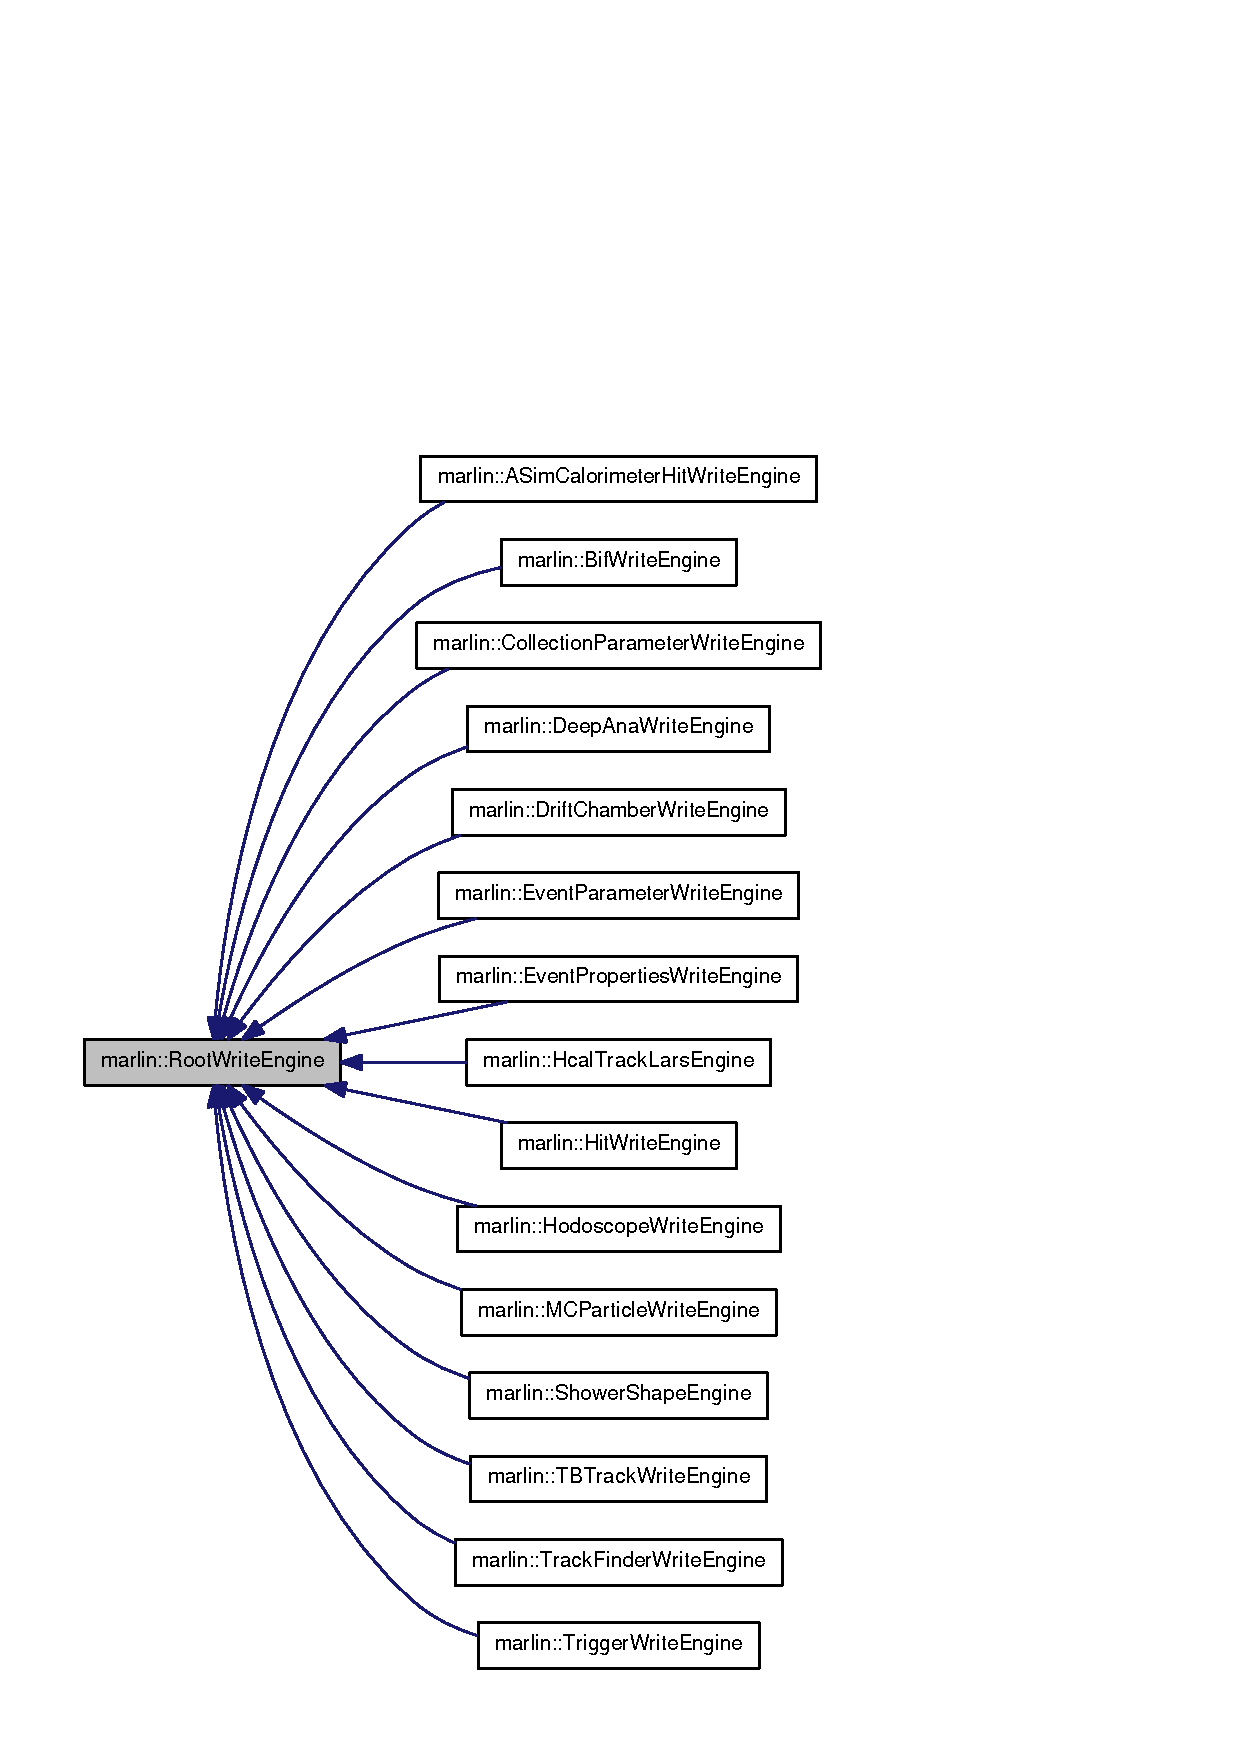
\includegraphics[height=400pt]{classmarlin_1_1RootWriteEngine__inherit__graph}
\end{center}
\end{figure}
Collaboration diagram for marlin::RootWriteEngine:\nopagebreak
\begin{figure}[H]
\begin{center}
\leavevmode
\includegraphics[width=232pt]{classmarlin_1_1RootWriteEngine__coll__graph}
\end{center}
\end{figure}
\subsection*{Public Member Functions}
\begin{DoxyCompactItemize}
\item 
{\bf RootWriteEngine} ({\bf RootTreeWriter} $\ast$host)
\item 
virtual const std::string \& {\bf getEngineName} ()=0
\item 
virtual void {\bf registerParameters} ()=0
\item 
virtual void {\bf registerBranches} (TTree $\ast$)=0
\item 
virtual void {\bf fillVariables} (EVENT::LCEvent $\ast$evt)=0
\end{DoxyCompactItemize}
\subsection*{Protected Attributes}
\begin{DoxyCompactItemize}
\item 
{\bf RootTreeWriter} \& {\bfseries \_\-hostProcessor}\label{classmarlin_1_1RootWriteEngine_ab53e690ff0f758b27f4ef45b87f3d3ce}

\end{DoxyCompactItemize}


\subsection{Detailed Description}
Abstract base class of callback classes for the RootTreeWrite processor Abstract interface for a RootTreeWriter-\/engine. Implement an descendant of this class to add variables to the output tree of the RootTreeWriterProcessor. After that add the new {\itshape engine\/} to the list of writer engines in the \doxyref{RootTreeWriter}{p.}{classmarlin_1_1RootTreeWriter} processor 

Definition at line 29 of file RootWriteEngine.hh.

\subsection{Constructor \& Destructor Documentation}
\index{marlin::RootWriteEngine@{marlin::RootWriteEngine}!RootWriteEngine@{RootWriteEngine}}
\index{RootWriteEngine@{RootWriteEngine}!marlin::RootWriteEngine@{marlin::RootWriteEngine}}
\subsubsection[{RootWriteEngine}]{\setlength{\rightskip}{0pt plus 5cm}marlin::RootWriteEngine::RootWriteEngine ({\bf RootTreeWriter} $\ast$ {\em host})\hspace{0.3cm}{\ttfamily  [inline]}}\label{classmarlin_1_1RootWriteEngine_a9a2f783fbd71d43487cb94feee09210a}
constructor 
\begin{DoxyParams}{Parameters}
\item[\mbox{$\leftarrow$} {\em host}]pointer to the \doxyref{RootTreeWriter}{p.}{classmarlin_1_1RootTreeWriter} processor the constructor of a derived class must pass this pointer to this base class e.g. \begin{DoxyVerb}
    /// SomeeWriteEngine( RootTreeWriter* host ):RootWriteEngine(host),
    ///                                          _engineName("SomeWriteEngine")
    /// {} \end{DoxyVerb}
 \end{DoxyParams}


Definition at line 38 of file RootWriteEngine.hh.

\subsection{Member Function Documentation}
\index{marlin::RootWriteEngine@{marlin::RootWriteEngine}!fillVariables@{fillVariables}}
\index{fillVariables@{fillVariables}!marlin::RootWriteEngine@{marlin::RootWriteEngine}}
\subsubsection[{fillVariables}]{\setlength{\rightskip}{0pt plus 5cm}virtual void marlin::RootWriteEngine::fillVariables (EVENT::LCEvent $\ast$ {\em evt})\hspace{0.3cm}{\ttfamily  [pure virtual]}}\label{classmarlin_1_1RootWriteEngine_ace823bd839cee7e8c8755e60c4cc7134}
Implement this to extract the variables which you want to fill into the {\itshape ROOT\/} tree from the event. Write the value of the variables you want to add to the tree to the member variables, which you registered to the {\itshape ROOT\/} tree. The \doxyref{RootTreeWriter}{p.}{classmarlin_1_1RootTreeWriter} will call TTree::Fill() for you. 
\begin{DoxyParams}{Parameters}
\item[{\em evt}]the current event \end{DoxyParams}


Implemented in {\bf marlin::EventPropertiesWriteEngine} \doxyref{}{p.}{classmarlin_1_1EventPropertiesWriteEngine_abc2305e78939db762a4c83bf669fe952}, {\bf marlin::ASimCalorimeterHitWriteEngine} \doxyref{}{p.}{classmarlin_1_1ASimCalorimeterHitWriteEngine_a23a4c30ce18b277e5dc5150775633d12}, {\bf marlin::BifWriteEngine} \doxyref{}{p.}{classmarlin_1_1BifWriteEngine_a5945f044afb17e832cf63380d3aa4330}, {\bf marlin::CollectionParameterWriteEngine} \doxyref{}{p.}{classmarlin_1_1CollectionParameterWriteEngine_a276cbc4b3fb6a51d52b7ff677cbe60ad}, {\bf marlin::DeepAnaWriteEngine} \doxyref{}{p.}{classmarlin_1_1DeepAnaWriteEngine_a9cf77605dc60b01d00169c80c2df921d}, {\bf marlin::DriftChamberWriteEngine} \doxyref{}{p.}{classmarlin_1_1DriftChamberWriteEngine_ae4ac9d60684437fd6b4d5c3365c0e7ef}, {\bf marlin::EventParameterWriteEngine} \doxyref{}{p.}{classmarlin_1_1EventParameterWriteEngine_ad9ccfdb2f6596c2ae60e6408ad011832}, {\bf marlin::HcalTrackLarsEngine} \doxyref{}{p.}{classmarlin_1_1HcalTrackLarsEngine_a3f7f7a652c8bc019dc0a9b069a2c6fce}, {\bf marlin::HitWriteEngine} \doxyref{}{p.}{classmarlin_1_1HitWriteEngine_a1ee46edbad4693ee7213c153c30dd2d9}, {\bf marlin::HodoscopeWriteEngine} \doxyref{}{p.}{classmarlin_1_1HodoscopeWriteEngine_a4db5d7173b75c3a59d2a8ae86fb0de93}, {\bf marlin::MCParticleWriteEngine} \doxyref{}{p.}{classmarlin_1_1MCParticleWriteEngine_aed3f0a8d52f56cbd1f3f4b93bad9670e}, {\bf marlin::ShowerShapeEngine} \doxyref{}{p.}{classmarlin_1_1ShowerShapeEngine_a02d946fe7bb758c32cff7206109d6882}, {\bf marlin::TBTrackWriteEngine} \doxyref{}{p.}{classmarlin_1_1TBTrackWriteEngine_a5250f4b00f85aabc3be6cff9593dae0f}, {\bf marlin::TrackFinderWriteEngine} \doxyref{}{p.}{classmarlin_1_1TrackFinderWriteEngine_a27566057dc6963c0fb0a5b3f779d6197}, and {\bf marlin::TriggerWriteEngine} \doxyref{}{p.}{classmarlin_1_1TriggerWriteEngine_a6b1216c91a9acbd4f4e09b7d45f3c8f7}.\index{marlin::RootWriteEngine@{marlin::RootWriteEngine}!getEngineName@{getEngineName}}
\index{getEngineName@{getEngineName}!marlin::RootWriteEngine@{marlin::RootWriteEngine}}
\subsubsection[{getEngineName}]{\setlength{\rightskip}{0pt plus 5cm}virtual const std::string\& marlin::RootWriteEngine::getEngineName ()\hspace{0.3cm}{\ttfamily  [pure virtual]}}\label{classmarlin_1_1RootWriteEngine_a31e38120fe60efcb15666fd569ba5862}
Returns the name of the engine to the \doxyref{RootTreeWriter}{p.}{classmarlin_1_1RootTreeWriter} processor. \begin{DoxyReturn}{Returns}
Must return a string with the engine name. 
\end{DoxyReturn}
\begin{Desc}
\item[{\bf Todo}]fixme: should be const, but must be declared const in implementations too. Need to fix all existing engines?!? \end{Desc}


Implemented in {\bf marlin::EventPropertiesWriteEngine} \doxyref{}{p.}{classmarlin_1_1EventPropertiesWriteEngine_ad264b9da6bc60ebd375faa319689941a}, {\bf marlin::ASimCalorimeterHitWriteEngine} \doxyref{}{p.}{classmarlin_1_1ASimCalorimeterHitWriteEngine_a76af2d1c30ce8566f1dcfacf551ab3dc}, {\bf marlin::BifWriteEngine} \doxyref{}{p.}{classmarlin_1_1BifWriteEngine_a82eecc72c7824876b9bb6211d9055e68}, {\bf marlin::CollectionParameterWriteEngine} \doxyref{}{p.}{classmarlin_1_1CollectionParameterWriteEngine_aec77b9403ff1661fd01d714b433157e8}, {\bf marlin::DeepAnaWriteEngine} \doxyref{}{p.}{classmarlin_1_1DeepAnaWriteEngine_a3b67cb94563a6f930a28f71bba8833c1}, {\bf marlin::DriftChamberWriteEngine} \doxyref{}{p.}{classmarlin_1_1DriftChamberWriteEngine_a54c3c6b481d7f957c95dc0b8dd9b9d37}, {\bf marlin::EventParameterWriteEngine} \doxyref{}{p.}{classmarlin_1_1EventParameterWriteEngine_a2a0b15f288547884438d616cba9a6ad0}, {\bf marlin::HcalTrackLarsEngine} \doxyref{}{p.}{classmarlin_1_1HcalTrackLarsEngine_a3d851ed89feec12237cb6c64a14cd54d}, {\bf marlin::HitWriteEngine} \doxyref{}{p.}{classmarlin_1_1HitWriteEngine_a13d17e1b000f55fd5819659426ece2f0}, {\bf marlin::HodoscopeWriteEngine} \doxyref{}{p.}{classmarlin_1_1HodoscopeWriteEngine_a18aa5f3029fd0fc951f8770afdf37f8a}, {\bf marlin::MCParticleWriteEngine} \doxyref{}{p.}{classmarlin_1_1MCParticleWriteEngine_a5cec023911524d85fb491a9a5d702ea0}, {\bf marlin::ShowerShapeEngine} \doxyref{}{p.}{classmarlin_1_1ShowerShapeEngine_ab379dcbe94700542c8a05c302d80231d}, {\bf marlin::TBTrackWriteEngine} \doxyref{}{p.}{classmarlin_1_1TBTrackWriteEngine_ab7ff50302fa10ce40cd78cd87472d1fd}, {\bf marlin::TrackFinderWriteEngine} \doxyref{}{p.}{classmarlin_1_1TrackFinderWriteEngine_a195ec04e9898f5436d1da6ba98886e44}, and {\bf marlin::TriggerWriteEngine} \doxyref{}{p.}{classmarlin_1_1TriggerWriteEngine_a6401f2bbd2a05725c55c851a0e4fcf39}.

Referenced by \_\-\_\-RTW::EngineRegistrar::appendAllEngines().\index{marlin::RootWriteEngine@{marlin::RootWriteEngine}!registerBranches@{registerBranches}}
\index{registerBranches@{registerBranches}!marlin::RootWriteEngine@{marlin::RootWriteEngine}}
\subsubsection[{registerBranches}]{\setlength{\rightskip}{0pt plus 5cm}virtual void marlin::RootWriteEngine::registerBranches (TTree $\ast$)\hspace{0.3cm}{\ttfamily  [pure virtual]}}\label{classmarlin_1_1RootWriteEngine_ad467dc6e73fdd9fd4311f7277fd02a89}
Implement to register local variables to the output tree 
\begin{DoxyParams}{Parameters}
\item[{\em pointer}]to the {\itshape ROOT\/} tree, which the \doxyref{RootTreeWriter}{p.}{classmarlin_1_1RootTreeWriter} processor fills at the end of each event. Usually the implementation looks like \begin{DoxyVerb}
    /// hostTree->Branch("variable",&_variable" ,"variable/F"  );
    /// \end{DoxyVerb}
. But you can add any type of branch you like. \end{DoxyParams}


Implemented in {\bf marlin::EventPropertiesWriteEngine} \doxyref{}{p.}{classmarlin_1_1EventPropertiesWriteEngine_a4c1282d1d34392d66b56de4d7efc6be8}, {\bf marlin::ASimCalorimeterHitWriteEngine} \doxyref{}{p.}{classmarlin_1_1ASimCalorimeterHitWriteEngine_a59a711512fa1cb7f0c3eb39a63af883d}, {\bf marlin::BifWriteEngine} \doxyref{}{p.}{classmarlin_1_1BifWriteEngine_a7589d618bd6113f426333a1aede37855}, {\bf marlin::CollectionParameterWriteEngine} \doxyref{}{p.}{classmarlin_1_1CollectionParameterWriteEngine_afd2c829f35e899f90f881a37aef206f9}, {\bf marlin::DeepAnaWriteEngine} \doxyref{}{p.}{classmarlin_1_1DeepAnaWriteEngine_afa0d65f082b588ef7d61c06aecd9afe4}, {\bf marlin::DriftChamberWriteEngine} \doxyref{}{p.}{classmarlin_1_1DriftChamberWriteEngine_a3b32b9dc07adaa637821917ec5a879a3}, {\bf marlin::EventParameterWriteEngine} \doxyref{}{p.}{classmarlin_1_1EventParameterWriteEngine_ad3a5361c939e7fccab20dc2b334aa33d}, {\bf marlin::HcalTrackLarsEngine} \doxyref{}{p.}{classmarlin_1_1HcalTrackLarsEngine_a5599070ef51668116f4287688f8e62a4}, {\bf marlin::HitWriteEngine} \doxyref{}{p.}{classmarlin_1_1HitWriteEngine_a9de31f39b17a9e782cc7d41d07fce547}, {\bf marlin::HodoscopeWriteEngine} \doxyref{}{p.}{classmarlin_1_1HodoscopeWriteEngine_ac106fb65ad09c7f41975ae5c355da9d2}, {\bf marlin::MCParticleWriteEngine} \doxyref{}{p.}{classmarlin_1_1MCParticleWriteEngine_abc8a55ab829d32228993664ee2fd084e}, {\bf marlin::ShowerShapeEngine} \doxyref{}{p.}{classmarlin_1_1ShowerShapeEngine_aa9b11fb1cee4af0d4dc90a687932c341}, {\bf marlin::TBTrackWriteEngine} \doxyref{}{p.}{classmarlin_1_1TBTrackWriteEngine_a7eeb8a39b0a40bfb13a0d1deb9c143cc}, {\bf marlin::TrackFinderWriteEngine} \doxyref{}{p.}{classmarlin_1_1TrackFinderWriteEngine_aa3fc66248aa14982aacea68e5b67f02e}, and {\bf marlin::TriggerWriteEngine} \doxyref{}{p.}{classmarlin_1_1TriggerWriteEngine_aa83e89d82bb8bc208b02d12d227e2bcb}.\index{marlin::RootWriteEngine@{marlin::RootWriteEngine}!registerParameters@{registerParameters}}
\index{registerParameters@{registerParameters}!marlin::RootWriteEngine@{marlin::RootWriteEngine}}
\subsubsection[{registerParameters}]{\setlength{\rightskip}{0pt plus 5cm}virtual void marlin::RootWriteEngine::registerParameters ()\hspace{0.3cm}{\ttfamily  [pure virtual]}}\label{classmarlin_1_1RootWriteEngine_ae12b70923768043fa5c1438f078c41d3}
Used to register steering parameters. Implement to register {\itshape \doxyref{marlin}{p.}{namespacemarlin}\/} steering file parameters. Use {\itshape \doxyref{marlin}{p.}{namespacemarlin}\/} syntax to register parameters for the calling \doxyref{RootTreeWriter}{p.}{classmarlin_1_1RootTreeWriter} processor.

use \begin{DoxyVerb}
    /// _hostProc.relayRegisterProcessorParameter(...)
    /// _hostProc.relayRegister...()
    /// \end{DoxyVerb}
 instead of {\itshape \doxyref{marlin}{p.}{namespacemarlin}\/} processors \begin{DoxyVerb}register...() \end{DoxyVerb}
 methods 

Implemented in {\bf marlin::EventPropertiesWriteEngine} \doxyref{}{p.}{classmarlin_1_1EventPropertiesWriteEngine_a9394c4461b767c0f763d087988e8c854}, {\bf marlin::ASimCalorimeterHitWriteEngine} \doxyref{}{p.}{classmarlin_1_1ASimCalorimeterHitWriteEngine_a5ad32bcf2f6723033b5a543a715f4d3c}, {\bf marlin::BifWriteEngine} \doxyref{}{p.}{classmarlin_1_1BifWriteEngine_a2f0940793cbb3314fe21843f9bde321b}, {\bf marlin::CollectionParameterWriteEngine} \doxyref{}{p.}{classmarlin_1_1CollectionParameterWriteEngine_ae5bd3085f961a8ecc90272f00886d7d8}, {\bf marlin::DeepAnaWriteEngine} \doxyref{}{p.}{classmarlin_1_1DeepAnaWriteEngine_a757be550fb07212cfbe8cd2a9d6e26be}, {\bf marlin::DriftChamberWriteEngine} \doxyref{}{p.}{classmarlin_1_1DriftChamberWriteEngine_a6632be0ed7f8ef14290e40550d64556c}, {\bf marlin::EventParameterWriteEngine} \doxyref{}{p.}{classmarlin_1_1EventParameterWriteEngine_a05d652e2a9398160729f20aa7d6cdd0d}, {\bf marlin::HcalTrackLarsEngine} \doxyref{}{p.}{classmarlin_1_1HcalTrackLarsEngine_a49bba2b5e26aafb89c9790f35175caae}, {\bf marlin::HitWriteEngine} \doxyref{}{p.}{classmarlin_1_1HitWriteEngine_a54f5c814d074396779ba6d21b2acff6c}, {\bf marlin::HodoscopeWriteEngine} \doxyref{}{p.}{classmarlin_1_1HodoscopeWriteEngine_ad5150110764a1bdd16c8a8eab05ef7bf}, {\bf marlin::MCParticleWriteEngine} \doxyref{}{p.}{classmarlin_1_1MCParticleWriteEngine_a18ac8b6f4d2818bf959ea494d1d17dae}, {\bf marlin::ShowerShapeEngine} \doxyref{}{p.}{classmarlin_1_1ShowerShapeEngine_a861065f4f0a4a91af65a700820cec207}, {\bf marlin::TBTrackWriteEngine} \doxyref{}{p.}{classmarlin_1_1TBTrackWriteEngine_a9ad2d4c87c6a35c554ed34ada4819678}, {\bf marlin::TrackFinderWriteEngine} \doxyref{}{p.}{classmarlin_1_1TrackFinderWriteEngine_a5c154e036f10b5ef6ed6673ec78e7598}, and {\bf marlin::TriggerWriteEngine} \doxyref{}{p.}{classmarlin_1_1TriggerWriteEngine_ae39e2db93985319eb4e8db5c1f6946b1}.

The documentation for this class was generated from the following file:\begin{DoxyCompactItemize}
\item 
RootWriteEngine.hh\end{DoxyCompactItemize}

\section{CALICE::TempRootTreeGenerator Class Reference}
\label{classCALICE_1_1TempRootTreeGenerator}\index{CALICE::TempRootTreeGenerator@{CALICE::TempRootTreeGenerator}}


Class to process Labview raw.  


{\ttfamily \#include $<$TempRootTreeGenerator.hh$>$}\subsection*{Public Member Functions}
\begin{DoxyCompactItemize}
\item 
virtual Processor $\ast$ {\bfseries newProcessor} ()\label{classCALICE_1_1TempRootTreeGenerator_a4683c88fa11fdadc38b174cbd78191df}

\item 
void {\bfseries init} ()\label{classCALICE_1_1TempRootTreeGenerator_a0a85ca935c8d4227cf78ff85745c801f}

\item 
void {\bfseries processEvent} (LCEvent $\ast$evt)\label{classCALICE_1_1TempRootTreeGenerator_affbf92f531b40ab279bec5764dd798b2}

\item 
void {\bfseries end} ()\label{classCALICE_1_1TempRootTreeGenerator_aebdde734f7d29091114a7c5da186e06f}

\item 
void {\bfseries registerBranches} (TTree $\ast$hostTree)\label{classCALICE_1_1TempRootTreeGenerator_a8c8c4c7c423b1aa404028e59960ba771}

\item 
void {\bfseries FillVariable} (LCEvent $\ast$evt)\label{classCALICE_1_1TempRootTreeGenerator_a3544386c3f78d68615da0c01f437e35e}

\end{DoxyCompactItemize}
\subsection*{Protected Attributes}
\begin{DoxyCompactItemize}
\item 
std::string {\bfseries \_\-inputColName}\label{classCALICE_1_1TempRootTreeGenerator_a08f763e65ab9a64986e987af8ce0117c}

\item 
std::string {\bfseries \_\-prefix}\label{classCALICE_1_1TempRootTreeGenerator_a324bde76149073163629a7e9e50c453e}

\item 
TFile $\ast$ {\bfseries \_\-rootFile}\label{classCALICE_1_1TempRootTreeGenerator_add462b67e83bd77baed72038875a81a6}

\item 
std::string {\bfseries \_\-rootFileName}\label{classCALICE_1_1TempRootTreeGenerator_a0c8aec17e8952dd62d3bfa678ce3eca3}

\item 
TTree $\ast$ {\bfseries \_\-treeTempSensorBlock}\label{classCALICE_1_1TempRootTreeGenerator_a40cc9d843dbba86306d56dbee9218c79}

\item 
\begin{tabbing}
xx\=xx\=xx\=xx\=xx\=xx\=xx\=xx\=xx\=\kill
struct \{\\
\>int {\bfseries nLayers}\\
\>float {\bfseries T1} [MAXPORTS]\\
\>float {\bfseries T2} [MAXPORTS]\\
\>float {\bfseries T3} [MAXPORTS]\\
\>float {\bfseries T4} [MAXPORTS]\\
\>float {\bfseries T5} [MAXPORTS]\\
\>float {\bfseries T6} [MAXPORTS]\\
\>float {\bfseries TDIF} [MAXPORTS]\\
\>float {\bfseries TPWR} [MAXPORTS]\\
\} {\bfseries \_hFill}\label{classCALICE_1_1TempRootTreeGenerator_ab47c17d8cd4b84b14b8912cf62281b5a}
\\

\end{tabbing}\end{DoxyCompactItemize}
\subsection*{Static Protected Attributes}
\begin{DoxyCompactItemize}
\item 
static const unsigned int {\bfseries MAXPORTS} = 1000\label{classCALICE_1_1TempRootTreeGenerator_ab2162b267c9e1f26729de736c4b2bf8d}

\end{DoxyCompactItemize}
\subsection*{Private Attributes}
\begin{DoxyCompactItemize}
\item 
int {\bfseries runNumber}\label{classCALICE_1_1TempRootTreeGenerator_ab6b2729ac1b292d2ee2fea66a9594703}

\item 
int {\bfseries eventNumber}\label{classCALICE_1_1TempRootTreeGenerator_a9d25e5c9fd0dbb2f75e1a3e149e45169}

\item 
long64 {\bfseries Timestamp}\label{classCALICE_1_1TempRootTreeGenerator_a987d676226994b2120f47c457551ba09}

\end{DoxyCompactItemize}
\subsection*{Static Private Attributes}
\begin{DoxyCompactItemize}
\item 
static std::map$<$ TTree $\ast$, {\bf TempRootTreeGenerator} $\ast$ $>$ {\bfseries \_\-treeFillerMap}\label{classCALICE_1_1TempRootTreeGenerator_a5aecfdab878099a4ea0a74e4b96652de}

\item 
static std::map$<$ TTree $\ast$, {\bf TempRootTreeGenerator} $\ast$ $>$ {\bfseries \_\-treeOwnerMap}\label{classCALICE_1_1TempRootTreeGenerator_a991022195e98911f7e5674c9ad674cce}

\item 
static std::map$<$ TFile $\ast$, {\bf TempRootTreeGenerator} $\ast$ $>$ {\bfseries \_\-fileOwnerMap}\label{classCALICE_1_1TempRootTreeGenerator_acf9f072ece6ac7300b4a6ef878bdb947}

\item 
static const double {\bfseries INVALID} = -\/FLT\_\-MAX\label{classCALICE_1_1TempRootTreeGenerator_ab51bc9fd4548675bdad7f48208a3c943}

\end{DoxyCompactItemize}


\subsection{Detailed Description}
Class to process Labview raw. \begin{DoxyAuthor}{Author}
: Shaojun Lu DESY 
\end{DoxyAuthor}
\begin{DoxyDate}{Date}
Nov 15 2012 
\end{DoxyDate}


Definition at line 20 of file TempRootTreeGenerator.hh.

The documentation for this class was generated from the following files:\begin{DoxyCompactItemize}
\item 
TempRootTreeGenerator.hh\item 
TempRootTreeGenerator.cc\end{DoxyCompactItemize}

\section{CALICE::TempSensorBlock Class Reference}
\label{classCALICE_1_1TempSensorBlock}\index{CALICE::TempSensorBlock@{CALICE::TempSensorBlock}}


Class for the Labview Data as acquired by the AHCAL Labview.  


{\ttfamily \#include $<$TempSensorBlock.hh$>$}\subsection*{Public Member Functions}
\begin{DoxyCompactItemize}
\item 
{\bf TempSensorBlock} (int TempSensorNumber, float TempSensorValue)\label{classCALICE_1_1TempSensorBlock_a5577684f2bdde7b3a3f201638f0aaf7a}

\begin{DoxyCompactList}\small\item\em Convenient c'tor. \item\end{DoxyCompactList}\item 
{\bf TempSensorBlock} (LCObject $\ast$obj)\label{classCALICE_1_1TempSensorBlock_ae45af5d892fd90492c15584eb1694190}

\begin{DoxyCompactList}\small\item\em 'Copy constructor' needed to interpret LCCollection read from file/database. \item\end{DoxyCompactList}\item 
virtual {\bf $\sim$TempSensorBlock} ()\label{classCALICE_1_1TempSensorBlock_aededba4f51f50d3056d76a31a97ec1ac}

\begin{DoxyCompactList}\small\item\em Important for memory handling. \item\end{DoxyCompactList}\item 
int {\bfseries GetTempSensorNumber} () const \label{classCALICE_1_1TempSensorBlock_af99dd00f4a3450d25eaa8b2bcb1e2b38}

\item 
float {\bfseries GetTempSensorValue} () const \label{classCALICE_1_1TempSensorBlock_a1485ee33033ab3a99c2ee8d3e5273138}

\item 
void {\bfseries print} (std::ostream \&os, int)\label{classCALICE_1_1TempSensorBlock_af1650378e195b324cfddfa3c2feb9ce6}

\item 
const std::string {\bf getTypeName} () const \label{classCALICE_1_1TempSensorBlock_a00a31b0c70354ed04a4bddc7d62772f3}

\begin{DoxyCompactList}\small\item\em Return the type of the class. \item\end{DoxyCompactList}\item 
const std::string {\bf getDataDescription} () const \label{classCALICE_1_1TempSensorBlock_ab9a8cfa10c171003da2614fb4518b566}

\begin{DoxyCompactList}\small\item\em Return a brief description of the data members. \item\end{DoxyCompactList}\end{DoxyCompactItemize}


\subsection{Detailed Description}
Class for the Labview Data as acquired by the AHCAL Labview. The class reflects that the data are received in the Labview \begin{DoxyAuthor}{Author}
S. Lu DESY Hamburg 
\end{DoxyAuthor}
\begin{DoxyDate}{Date}
Dec 17 2012 
\end{DoxyDate}


Definition at line 23 of file TempSensorBlock.hh.

The documentation for this class was generated from the following file:\begin{DoxyCompactItemize}
\item 
TempSensorBlock.hh\end{DoxyCompactItemize}

\section{CALICE::TempSensorBlock2 Class Reference}
\label{classCALICE_1_1TempSensorBlock2}\index{CALICE::TempSensorBlock2@{CALICE::TempSensorBlock2}}


Class for the Labview Data as acquired by the AHCAL Labview.  


{\ttfamily \#include $<$TempSensorBlock2.hh$>$}\subsection*{Public Member Functions}
\begin{DoxyCompactItemize}
\item 
{\bf TempSensorBlock2} (int LDANumber, int PortNumber, int T1, int T2, int T3, int T4, int T5, int T6, int TDIF, int TPWR)\label{classCALICE_1_1TempSensorBlock2_a54e191771f53ca8f7cbb1515d7aca02f}

\begin{DoxyCompactList}\small\item\em Convenient c'tor. \item\end{DoxyCompactList}\item 
{\bf TempSensorBlock2} (LCObject $\ast$obj)\label{classCALICE_1_1TempSensorBlock2_a38018a53d6021897d93a8c5dceb4d414}

\begin{DoxyCompactList}\small\item\em 'Copy constructor' needed to interpret LCCollection read from file/database. \item\end{DoxyCompactList}\item 
virtual {\bf $\sim$TempSensorBlock2} ()\label{classCALICE_1_1TempSensorBlock2_af5f34f2ff55c040772d6608011f215be}

\begin{DoxyCompactList}\small\item\em Important for memory handling. \item\end{DoxyCompactList}\item 
int {\bfseries GetLDANumber} () const \label{classCALICE_1_1TempSensorBlock2_a13a5db490dd71b4986d7f9a9f8305ed5}

\item 
int {\bfseries GetPortNumber} () const \label{classCALICE_1_1TempSensorBlock2_ac954ae46175ebe0fc480e4961645149a}

\item 
int {\bfseries GetT1} () const \label{classCALICE_1_1TempSensorBlock2_aec4184305621faf41a9ad39a0b70eb34}

\item 
int {\bfseries GetT2} () const \label{classCALICE_1_1TempSensorBlock2_a910deb622a4882de3c245cdd74a792ed}

\item 
int {\bfseries GetT3} () const \label{classCALICE_1_1TempSensorBlock2_abec6d13fe16bb8e9afabbd7eabdc0dbc}

\item 
int {\bfseries GetT4} () const \label{classCALICE_1_1TempSensorBlock2_a8689abf3279957fe644cf450ee08ddc8}

\item 
int {\bfseries GetT5} () const \label{classCALICE_1_1TempSensorBlock2_a9f6702c33d6e3813b1d2b24b918d8d82}

\item 
int {\bfseries GetT6} () const \label{classCALICE_1_1TempSensorBlock2_a54d82a9b7521b8d9483ee600c1ad375f}

\item 
int {\bfseries GetTDIF} () const \label{classCALICE_1_1TempSensorBlock2_a833e1b88513124ae5370c2777dfa0bdd}

\item 
int {\bfseries GetTPWR} () const \label{classCALICE_1_1TempSensorBlock2_a9120824274d48a1a77218219de1139da}

\item 
void {\bfseries print} (std::ostream \&os, int)\label{classCALICE_1_1TempSensorBlock2_a18fcad9b01f87d568216df1198423cff}

\item 
const std::string {\bf getTypeName} () const \label{classCALICE_1_1TempSensorBlock2_aa7c390c29411439dbd83bd24f639570d}

\begin{DoxyCompactList}\small\item\em Return the type of the class. \item\end{DoxyCompactList}\item 
const std::string {\bf getDataDescription} () const \label{classCALICE_1_1TempSensorBlock2_a876ddbe948463b85208e29cc03fc894b}

\begin{DoxyCompactList}\small\item\em Return a brief description of the data members. \item\end{DoxyCompactList}\end{DoxyCompactItemize}


\subsection{Detailed Description}
Class for the Labview Data as acquired by the AHCAL Labview. The class reflects that the data are received in the Labview \begin{DoxyAuthor}{Author}
S. Lu DESY Hamburg 
\end{DoxyAuthor}
\begin{DoxyDate}{Date}
Dec 17 2012 
\end{DoxyDate}


Definition at line 23 of file TempSensorBlock2.hh.

The documentation for this class was generated from the following file:\begin{DoxyCompactItemize}
\item 
TempSensorBlock2.hh\end{DoxyCompactItemize}

\section{CALICE::TempSensorBlockOld Class Reference}
\label{classCALICE_1_1TempSensorBlockOld}\index{CALICE::TempSensorBlockOld@{CALICE::TempSensorBlockOld}}


Class for the Labview Data as acquired by the AHCAL Labview.  


{\ttfamily \#include $<$TempSensorBlockOld.hh$>$}\subsection*{Public Member Functions}
\begin{DoxyCompactItemize}
\item 
{\bf TempSensorBlockOld} (float layer, float T1, float T2, float T3, float T4, float T5, float T6, float TDIF, float TPWR)\label{classCALICE_1_1TempSensorBlockOld_a82d44ba02d686f455a449b7973a84458}

\begin{DoxyCompactList}\small\item\em Convenient c'tor. \item\end{DoxyCompactList}\item 
{\bf TempSensorBlockOld} (LCObject $\ast$obj)\label{classCALICE_1_1TempSensorBlockOld_a8fa3c63309c635a015babba9cd9bcc5e}

\begin{DoxyCompactList}\small\item\em 'Copy constructor' needed to interpret LCCollection read from file/database. \item\end{DoxyCompactList}\item 
virtual {\bf $\sim$TempSensorBlockOld} ()\label{classCALICE_1_1TempSensorBlockOld_aa38e40270950ded8526b545854977c3c}

\begin{DoxyCompactList}\small\item\em Important for memory handling. \item\end{DoxyCompactList}\item 
float {\bfseries GetLayer} () const \label{classCALICE_1_1TempSensorBlockOld_ae6bf017ac104815ba921e869d089b995}

\item 
float {\bfseries GetT1} () const \label{classCALICE_1_1TempSensorBlockOld_a5a7ed17b117faae8ac76b9cc96e13296}

\item 
float {\bfseries GetT2} () const \label{classCALICE_1_1TempSensorBlockOld_a4663dda7309826ace2cf5bd61b67e5e0}

\item 
float {\bfseries GetT3} () const \label{classCALICE_1_1TempSensorBlockOld_af4a3ebf85837357ca3f779c4f76aec2a}

\item 
float {\bfseries GetT4} () const \label{classCALICE_1_1TempSensorBlockOld_a9d33ccb66b6ecc6fd9b09dc3ec74b05e}

\item 
float {\bfseries GetT5} () const \label{classCALICE_1_1TempSensorBlockOld_aa3e9bc414a3bb44caf97fcc815417790}

\item 
float {\bfseries GetT6} () const \label{classCALICE_1_1TempSensorBlockOld_af20c1b20fbd07c01f80ce2e9ad1ec03b}

\item 
float {\bfseries GetTDIF} () const \label{classCALICE_1_1TempSensorBlockOld_a5b6390ec23ce91e080f94188ecf2708f}

\item 
float {\bfseries GetTPWR} () const \label{classCALICE_1_1TempSensorBlockOld_a71713df3906fbd95f628d58d53c233f7}

\item 
void {\bfseries print} (std::ostream \&os, float)\label{classCALICE_1_1TempSensorBlockOld_afbe6d02c5fa6af5dedc8269ac47d3e53}

\item 
const std::string {\bf getTypeName} () const \label{classCALICE_1_1TempSensorBlockOld_aeeed0bef453e6e628add8cdc206febc0}

\begin{DoxyCompactList}\small\item\em Return the type of the class. \item\end{DoxyCompactList}\item 
const std::string {\bf getDataDescription} () const \label{classCALICE_1_1TempSensorBlockOld_a1a0946cac03450c5f658780aee2c3ee6}

\begin{DoxyCompactList}\small\item\em Return a brief description of the data members. \item\end{DoxyCompactList}\end{DoxyCompactItemize}


\subsection{Detailed Description}
Class for the Labview Data as acquired by the AHCAL Labview. The class reflects that the data are received in the Labview \begin{DoxyAuthor}{Author}
S. Lu DESY Hamburg 
\end{DoxyAuthor}
\begin{DoxyDate}{Date}
Dec 17 2012 
\end{DoxyDate}


Definition at line 24 of file TempSensorBlockOld.hh.

The documentation for this class was generated from the following file:\begin{DoxyCompactItemize}
\item 
TempSensorBlockOld.hh\end{DoxyCompactItemize}

\printindex
\end{document}
